\documentclass{jknotes} % scrartcl with extras
\usepackage{joshkirklin}

\begin{document}

\institution{Cambrige Part III Maths}
\title{Quantum Field Theory}
\lecturer{Malcolm Perry}
\notetaker{Josh Kirklin}
\date{Michaelmas 2015}

\maketitle
\suggestionsspiel

\tableofcontents

\section{Introduction}
In these notes we will use natural units: \(\hbar = c = 1\), \([L]=[T]=[M]^{-1}\).

\subsection{Why study QFT?}

There are many reasons to study Quantum Field Theory.
\begin{itemize}
    \item QFT provides a way to unify special relativity with quantum mechanics.
    \item Using QFT, we can understand what spin is and how it works. For example we can deduce the reason why bosons have Bose-Einstein statistics, and fermions have Fermi-Dirac statistics.
    \item QFT enables us to explain why particles exist, and furthermore why they can morph into different forms over time. In other words, we can analyse the reactions between various species of particle, for example electron positron annihilation: \(e^+e^-\rightarrow2\gamma\).
    \item The ``Rayleigh-Jeans catastrophe'' is a problem that arises in dealing with the electromagnetic field. In simple terms the problem is that a certain law predicts divergences at high energies. With QFT we can solve this problem and other more general ultraviolet divergences.
    \item QFT provides a theoretical framework for describing and studying all fundamental processes\footnote{Except of course for gravitation. For that we require something else; String Theory for instance.}. The best theory for our world that we have today is the \emph{Standard Model}, which has experimentally been found to accurately describe electromagnetic, weak and strong interactions to five decimal places.
\end{itemize}

\subsection{Special relativity}

\begin{defn}
    \emph{Minkowski spacetime} \(\RR^{3,1}\) is a four-dimensional space equipped with the Minkowski metric \(\eta = \operatorname{diag}(-1,1,1,1)\).
\end{defn}

The geometry of Minkowski spacetime is described by its line element:
\begin{equation}
    \dd{s^2} = \eta_{ab} \dd{x^a} \dd{x^b} = -\dd{t^2}+\dd{x^2}+\dd{y^2}+\dd{z^2}
\end{equation}
In rough terms, \(\dd{s}\) is the ``distance'' between the infinitesimally close points \((t,x,y,z)\) and \((t+\dd{t},x+\dd{x},y+\dd{y},z+\dd{z})\).

Vectors in Minkowski space can be classified into five different types, depending on their relation to the lightcone, i.e.\ the locus of all points \(x^a\) with \(\eta_{ab}x^ax^b = x \cdot x = |x|^2 = 0\).

\begin{minipage}{0.39\linewidth}
    \begin{figure}[H]
        \raggedleft
        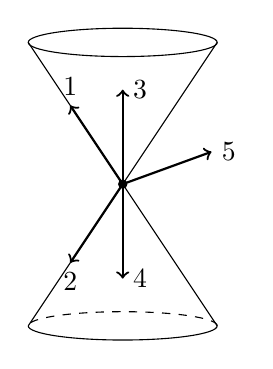
\begin{tikzpicture}[scale=0.6]
            \draw (2,3) -- (-2,-3);
            \draw (2,-3) -- (-2,3);
            \draw[yscale=0.15,dashed] (2,-20) arc (0:180:2);
            \draw[yscale=0.15] (-2,-20) arc (180:360:2);
            \draw[yscale=0.15] (0,20) circle (2);
            \fill (0,0) circle (0.1);
            \draw[thick,->] (0,0) -- ({-4/sqrt(13)},{6/sqrt(13)}) node[above] {\(1\)};
            \draw[thick,->] (0,0) -- ({-4/sqrt(13)},{-6/sqrt(13)}) node[below] {\(2\)};
            \draw[thick,->] (0,0) -- (0,2) node[right] {\(3\)};
            \draw[thick,->] (0,0) -- (0,-2) node[right] {\(4\)};
            \draw[thick,->] (0,0) -- ({2*cos(20)},{2*sin(20)}) node[right] {\(5\)};
        \end{tikzpicture}
    \end{figure}
\end{minipage}
\begin{minipage}{0.6\linewidth}
    \begin{enumerate}
        \item Future directed null vectors.
        \item Past directed null vectors.
        \item Future directed timelike vectors.
        \item Past directed timelike vectors.
        \item Spacelike vectors.
    \end{enumerate}
\end{minipage}


\begin{defn}
    A \emph{Lorentz transformation} is a transformation \(x \rightarrow x' = \Lambda x\) between \emph{inertial frames} such that \(\trans{\Lambda}\eta\Lambda=\eta\). We say that \(\Lambda\) preserves the Minkowski metric.
\end{defn}

\begin{eg}
    Suppose one wants to transform a rest frame to one moving at velocity \(v\) in the (positive) \(x\)-direction. Then we can use the following Lorentz transformation:
    \begin{align}
        t &\rightarrow t' = \frac{t-vx}{\sqrt{1-v^2}} \\
        x &\rightarrow x' = \frac{x-vt}{\sqrt{1-v^2}} \\
        y &\rightarrow y' = y \\
        z &\rightarrow z' = z
    \end{align}
\end{eg}

The set of all Lorentz transformations equipped with matrix multiplication form a group which we call the \emph{Lorentz group} \(SO(3,1)\):
\begin{itemize}
    \item Matrix multiplication is associative.
    \item Suppose \(\Lambda,\Lambda' \in SO(3,1)\). Then \(\trans{\Lambda\Lambda'}\eta\Lambda\Lambda' = \trans{\Lambda'}\trans{\Lambda}\eta\Lambda\Lambda' = \trans{\Lambda'}\eta\Lambda' = \eta\), so \(\Lambda\Lambda' \in SO(3,1)\), i.e. \(SO(3,1)\) is closed.
    \item The matrix identity \(\identity\) is an element of \(SO(3,1)\).
    \item Suppose \(\Lambda \in SO(3,1)\). Then taking the determinant of both sides of \(\trans{\Lambda}\eta\Lambda = \eta\) we obtain \(-(\det\Lambda)^2=-1\), so \(\det\Lambda \ne 0\) i.e. \(\Lambda\) is invertible. Moreover, if we left-multiply by \(\trans{\Lambda}^{-1}\) and right-multiply by \(\Lambda^{-1}\) we obtain \(\eta = \trans{\Lambda}^{-1}\eta\Lambda^{-1}\), so \(\Lambda^{-1} \in SO(3,1)\).
\end{itemize}

The Lorentz group contains spatial rotations. For example, a rotation of \(\theta\) about the \(x\)-axis is given by:
\begin{equation}
    \Lambda = 
    \begin{pmatrix}
        1 \\
        & \cos\theta & -\sin\theta \\
        & \sin\theta & \cos\theta \\
        &&& 1
    \end{pmatrix}
\end{equation}
More generally, a rotation of \(\theta\) about the direction given by a 3D unit vector \(n_i\) can be written:
\begin{equation}
    \Lambda = 
    \begin{pmatrix}
        1 \\
        & R
    \end{pmatrix}
    \qq{where}
    R_{ij} = \cos\theta\delta_{ij} + n_in_j(1-\cos\theta) - \epsilon_{ijk} n_k \sin \theta
\end{equation}
A \emph{Lorentz boost} is a shift in velocity between frames. The Lorentz boost with velocity shift given by a 3D vector \(v_i\) can be written:
\begin{equation}
    \Lambda = 
    \begin{pmatrix}
        \gamma & -\gamma v_i \\
        -\gamma v_j & \delta_{ij}+\frac{\gamma^2}{1+\gamma}v_iv_j
    \end{pmatrix}
    \qq{where}
    \gamma = (1-v_iv_i)^{-\frac{1}{2}}
\end{equation}

\begin{defn}
    A \emph{proper} Lorentz transformation \(\Lambda\) has \(\det\Lambda = 1\). An \emph{improper} Lorentz transformation \(\Lambda\) has \(\det\Lambda = -1\).
\end{defn}

Proper Lorentz transformations are continuously connected to the identity. Under a proper Lorentz transformation, the type (i.e.\ spacelike, future directed timelike, etc) of a vector is invariant. Both rotations and boosts are proper.

There are two types of improper Lorentz transformations:
\begin{itemize}
    \item \emph{Parity transformation}: \(\vec{x}\rightarrow-\vec{x}\).
    \item \emph{Time reversal}: \(t \rightarrow -t\).
\end{itemize}
Time reversal maps \(\left\{
\begin{matrix}
    \text{future} \\ \text{past}
\end{matrix}
\right\}\) directed vectors to \(\left\{
\begin{matrix}
    \text{past} \\ \text{future}
\end{matrix}
\right\}\) directed vectors.

The action of a Lorentz transform on spacetime co-ordinates is to take \(x^a \rightarrow \tilde{x}^a = \Lambda\indices{^a_b}x^b\), but other objects transform in other ways.

\begin{defn}
    An \(X\)-valued \emph{scalar field} is a field in spacetime \(S:\RR^{3,1}\rightarrow X\) that is invariant under Lorentz transformations:
    \begin{equation}
        S(x) \rightarrow \tilde{S}(\tilde{x}) = S(\Lambda x)
    \end{equation}
\end{defn}
\begin{defn}
    An \(X\)-valued \emph{covariant vector field} is a set of fields in spacetime \(\{V^a:\RR^{3,1}\rightarrow X\}\) that transform just like co-ordinates under Lorentz transforms:
    \begin{equation}
        V^a(x) \rightarrow \tilde{V}^a(\tilde{x}) = \Lambda\indices{^a_b}V^b(\Lambda x)
    \end{equation}
\end{defn}
In this course we will deal usually with fields that are \(\RR\) or \(\CC\)-valued.

Two vector fields can be combined into a scalar field by taking their inner product.

A useful convention is to swap the positions of indices upstairs or downstairs using the metric \(\eta\). E.g. \(W_a=\eta_{ab}W^b\) where \(W^b\) is a covariant vector. \(W_a\) is a \emph{contravariant vector} and is dual to \(W^b\). We also define \(\eta^{ab}=(\eta^{-1})_{ab}\). 

In index notation, we have for any Lorentz transformation \(\Lambda\):
\begin{equation}
    \Lambda\indices{^a_c}\Lambda\indices{^b_d}\eta_{ab}=\eta_{cd}
\end{equation}
Now pre-multiply by the inverse of \(\Lambda\):
\begin{equation}
    \underbrace{(\Lambda^{-1})\indices{^c_e}\Lambda\indices{^a_c}}_{=\delta^a_e} \eta_{ab} = (\Lambda^{-1})\indices{^c_e}\eta_{cd}
    \implies
    \Lambda\indices{^b_d} \eta_{eb} = (\Lambda^{-1})\indices{^c_e}\eta_{cd}
\end{equation}
Now post-multiply by an \(\eta\):
\begin{equation}
    \Lambda\indices{^b_d}\eta_{eb} \eta^{df} = (\Lambda^{-1})\indices{^c_e}\eta_{cd}\eta^{df} = (\Lambda^{-1})\indices{^f_e}
\end{equation}
So, since we are adopting the convention that any index can be raised or lowered using \(\eta\), we have:
\begin{equation}
    (\Lambda^{-1})\indices{^f_e}=\Lambda\indices{_e^f} \quad \text{i.e.} \quad \Lambda^{-1} = \trans{\Lambda}
\end{equation}
We can deduce how a contravariant tensor transforms:
\begin{equation}
    W_a \rightarrow \tilde{W}_a = \eta_{ab}\tilde{W}^b = \eta_{ab} \Lambda\indices{^b_c}W^c = \eta_{ab} \eta^{bd} \Lambda\indices{_d^e} \eta_{ec} W^c  = \Lambda\indices{_a^e} W_e
\end{equation}

\begin{defn}
    An \(X\)-valued \emph{tensor field of rank \((n,m)\)} is a set of fields \(\{T\indices{^{a_1\dots  a_n}_{b_1\dots b_m}} : \RR^{3,1} \rightarrow X\}\) that transform with \(n\) covariant indices and \(m\) contravariant indices, i.e.:
    \begin{equation}
        T\indices{^{a_1\dots}_{b_1\dots}} (x) \rightarrow \tilde{T}\indices{^{c_1\dots}_{d_1\dots}} (\tilde{x}) = \Lambda\indices{^{c_1}_{a_1}}\cdots\Lambda\indices{_{d_1}^{b_1}}\cdots T\indices{^{a_1\dots}_{b_1\dots}} (\Lambda x)
        \label{}
    \end{equation}
\end{defn}

\begin{defn}
    A \emph{symmetry} of Minkowski spacetime is a transformation that leaves the line element invariant. The group of symmetries of Minkowski spacetime is called the \emph{Poincar\'e group}.
\end{defn}

The Poincar\'e group includes Lorentz transformations as well as spacetime translations. In fact it is a 10-dimensional group:
\begin{itemize}
    \item 3 spatial rotations
    \item 3 Lorentz boosts
    \item 3 spatial translations
    \item 1 time translation
\end{itemize}
These 10 transformations correspond to the 10 Killing vectors of Minkowski space.

In Minkowski space in Cartesian coordinates the differential operators \(\partial_a = \pdv{x^a}\) map tensors of type \((n,m)\) to tensors of type \((n,m+1)\).

\subsection{Quantum mechanics}
When we quantise a classical theory, we convert classical observables into Hermitian operators. For example for a one particle system, we have an energy operator \(\hat{E} = i \pdv{t}\) and a momentum operator \(\hat{\vec{p}} = -i\grad\). Classically, energy and spatial momentum are combined into 4-momentum \(p\) given by:
\begin{equation}
    p^a = (\text{energy},\text{spatial momentum}) \qq{or equivalently} p_a = (-\text{energy},\text{spatial momentum})
\end{equation}
Thus we can define a 4-momentum operator \(\hat{p}_a=-i\partial_a\). In non-relativistic quantum mechanics, \(\hat{p}_i\) and \(\hat{x}^j\) obey the \emph{Heisenberg algebra}:
\begin{equation}
    [\hat{p}_i,\hat{x}^j] = -i\delta^j_i
\end{equation}
To make this relativistic, we simply include time coordinates, so we take \(\hat{p}_i \rightarrow \hat{p}_a\) and \(\hat{x}^j \rightarrow \hat{p}^b\):
\begin{equation}
    [\hat{p}_a,\hat{x}^b] = -i\delta^b_a \quad (\text{or}\, [\hat{p}_a,\hat{x}_b]=-i\eta_{ab} \,\text{etc.})
\end{equation}
Classically, we define the angular momentum with \(L_i = (\vec{x}\times\vec{y})_i = \epsilon_{ijk}x_jp_k\). But now we encounter problems in translating to relativistic quantum mechanics. Classically, the ordering of \(x_j,p_k\) does not matter, but quantumly the ordering of \(\hat{x}_j,\hat{p}_k\) does. Furthermore, \(\epsilon_{ijk}\) is a 3D alternating symbol, which does not fit with our 4D Minkowski spacetime. The way we get around these problems is to instead think of angular momentum as an antisymmetric tensor \(L_{ij} = x_ip_j-x_jp_i\), or in relativistic form \(L_{ab} = x_ap_b-p_ax_b\). Note that \(x_a\) and \(p_b\) only don't commute if \(a=b\), and because \(L_{ab}\) is antisymmetric, we need not worry about that case. So after quantisation we obtain:
\begin{equation}
    \hat{L}_{ab} = -i\hat{x}_a\partial_b + i\hat{x}_b\partial_a
\end{equation}
It is not hard to show that:
\begin{equation}
    [\hat{L}_{ab},\hat{L}_{cd}] = i( \hat{L}_{ad}\eta_{bc}-\hat{L}_{ac}\eta_{bd}-\hat{L}_{bd}\eta_{ac}+\hat{L}_{bc}\eta_{ad} )
\end{equation}
This is exactly the bracket structure for the Lie algebra of the Lorentz group \(\mathcal{L}(SO(3,1))\), so this shows that \(\hat{L}_{ab}\) forms a representation of \(\mathcal{L}(SO(3,1))\).

\section{Scalar Fields}

\subsection{Classical scalar fields}

Consider fields \(\phi(\vb{x},t)\) that are eigenstates of the momentum operator \(-i\partial_a\). It is easy to see that these are the \emph{plane wave} states \(\phi = e^{ik_ax^a}\) with eigenvalue \(k_a\). If \(k_a\) is a physical momentum, as it should be, then it is a contravariant vector. Thus \(k_ax^a\) is a scalar and so is \(\phi\).

Fourier transforms give a way of moving between spatial co-ordinates and relativistic momenta, \(\phi(x) \rightarrow \hat\phi(p)\):
\begin{equation}
    \hat\phi(p) = \int \dd[4]{x}\phi(x)e^{-ip_ax^a}
\end{equation}
where \(\dd[4]{x} = \dd[3]{x}\dd{t} = \prod_a\dd{x^a}\) and the integral is taken over all of spacetime. This has an exact inverse \(\hat\phi(p) \rightarrow \hat\phi(x)\):
\begin{equation}
    \phi(x) = \frac{1}{(2\pi)^4}\int\dd[4]{p}\hat\phi(p)e^{ip_ax^a}
\end{equation}
where \(\dd[4]{p} = \dd[3]{p}\dd{p^0} = \dd[3]{p}\dd{E} = \prod_a \dd{p^a}\) and the integral is taken over all 4-momenta.

The Fourier transform of a plane wave state is given by a delta function:
\begin{equation}
    \int\dd[4]{x}e^{ik_bx^b}e^{-ip_ax^a} = \int\dd[4]{x}e^{i(k_0-p_0)t + i(\vec{k}-\vec{p})\cdot\vec{x}} = (2\pi)^4\delta^{(4)}(k-p)
\end{equation}

In special relativity, the rest mass \(m\) of a particle is given by \(p^ap_a = -E^2+\vb{p}^2 = -m^2\). If we write this in terms of the momentum operator, we obtain the \emph{Klein-Gordon equation}:
\begin{equation}
    (-\dalembertian + m^2)\phi = 0
\end{equation}
where \(\dalembertian = \eta^{ab}\partial_a\partial_b = \pdv[2]{t} - \laplacian\) is the relativistic \emph{d'Alembertian} or \emph{wave operator}.
We will want the Klein-Gordon equation to be the equation of motion for our field, so it is natural to ask: is there a Lagrangian action to to reproduce it? The answer is yes, and the action is the \emph{Klein-Gordon action}:
\begin{equation}
    I = \int \dd[4]{x} \qty(-\frac{1}{2}\eta^{ab}\partial_a\phi\partial_b \phi- \frac{1}{2}m^2\phi^2)
\end{equation}
To verify that this is the case, let's vary \(I\) with regard to \(\phi\):
\begin{align}
    \var{I} &= \int \dd[4]{x} \qty(-\eta^{ab} \partial_a \var{\phi} \partial_a \phi - m^2 \phi \var{\phi}) \\
    &= \int \dd[4]{x} \underbrace{\qty(\eta^{ab} \partial_a\partial_b\phi - m^2\phi)}_\text{Klein-Gordon} \var{\phi}
    + \underbrace{\int \dd{\Sigma^a} \qty(\var{\phi}\partial_a\phi)}_\text{boundary term}
\end{align}
where we reach the second line by partial integration. In this course we will assume that all fields go to zero sufficiently quickly as we approach infinity, so the boundary term vanishes. Thus, since \(\var{\phi}\) is arbitrary, in order to satisfy \(\var{I}=0\) we must have \(\eta^{ab} \partial_a\partial_b\phi - m^2\phi = 0\), i.e.\ the Klein-Gordon equation must hold.

\subsection{Quantisation}

Lets summarise how classical dynamics progresses through the Hamiltonian formalism to quantum mechanics. In normal classical dynamics we have a (usually finite) set of generalised coordinates \(q_i\), labelled by \(i\). We define the generalised momenta \(\pi_i\) congugate to each coordinate \(q_i\) by:
\begin{equation}
    \pi_i = \pdv{L}{\dot{q}_i}
\end{equation}
We can solve this equation for \(\dot{q}_i\) as a function of the \(\pi_j\) and \(q_k\). We then define the Hamiltonian by:
\begin{equation}
    H(\pi_i,q_i) = \sum_i \pi_i \dot{q}_i(\pi_j,q_k) - L
\end{equation}
Given any observable \(X(\pi,q)\), its time evolution is given by:
\begin{equation}
    \dot{X} = \pb{X}{H}_P
\end{equation}
where the braced quantity is the \emph{Poisson bracket}, defined by:
\begin{equation}
    \pb{X}{Y}_P = \sum_i \pdv{X}{q_i}\pdv{Y}{\pi_i}-\pdv{X}{\pi_i}\pdv{Y}{q_i}
\end{equation}
Note that we have \(\pb{q_i}{\pi_j}_P = \delta_{ij}\).

To quantise, we must ``deform'' the classical system by replacing \(q\), \(\pi\) and other observables by Hermitian operators, and by replacing all Poisson brackets by a commutator:
\begin{equation}
    \pb{X}{Y}_P \rightarrow -i[\hat{X},\hat{Y}]
\end{equation}
For example, \(\pb{q_i}{\pi_j}_P = \delta_{ij}\) becomes \([\hat{q}_i,\hat\pi_j] = i\hbar\delta_{ij}\).

Now return to the scalar field. 
\begin{defn}
    The \emph{functional derivative} \(\fdv{F}{f}\) of a functional \(F[f]\) is defined in the following way:
    \begin{equation}
        \fdv{F[f(x)]}{f(y)} = \left. \pdv{\epsilon}F[f(x)+\epsilon\delta(x-y)] \right|_{\epsilon=0}
    \end{equation}
    where the delta function has the appropriate dimensionality.
\end{defn}
Functional derivatives follow all of the normal rules of derivatives (e.g.\ the chain rule and product rule). 

For example, for the Klein-Gordon action we have:
\begin{equation}
    \fdv{I}{\phi(x)} = \eta^{ab}\partial_a\partial_b \phi(x) - m^2 \phi(x)
\end{equation}

We view the action \(I\) as an integral over all time of a Lagrangian \(L(\phi,\dot\phi)\):

\begin{equation}
    I = \int\dd{t} L(\phi,\dot\phi) \qq{where} L(\phi,\dot\phi) = \int\dd[3]{x}\qty(\frac{1}{2}\dot\phi^2 - \frac{1}{2}\qty(\grad\phi)^2-\frac{1}{2}m^2\phi^2)
\end{equation}

In field theory, we have an infinite continuum of generalised co-ordinates \(\phi(\vb{x})\) labelled by points in space \(\vb{x}\).  In order to account for this, to produce a Hamiltonian formalism we use functional derivatives instead of partial derivatives.

\begin{defn}
    The momentum conjugate to a particular field \(\phi(\vb{x})\) with a Lagrangian \(L\) is given by:
    \begin{equation}
        \pi(\vb{x}) = \fdv{L}{\dot\phi(\vb{x})}
    \end{equation}
\end{defn}

For a scalar field obeying the Klein-Gordon equation, we have \(\pi(\vb{x}) = \dot\phi(\vb{x})\). The Hamiltonian \(H\) is given by:
\begin{equation}
    H = \int\dd[3]{x} \pi(\vb{x})\dot\phi(\vb{x}) - L
\end{equation}
For a scalar field obeying the Klein-Gordon equation, this becomes:
\begin{align}
    H &= \int\dd[3]{x} \pi(\vb{x})\dot\phi(\vb{x}) - \frac{1}{2} \dot\phi^2 + \frac{1}{2} (\grad\phi)^2 + \frac{1}{2}m^2\phi^2 \\
    &= \int\dd[3]{x} \frac{1}{2}\pi^2 + \frac{1}{2}(\grad\phi)^2 + \frac{1}{2}m^2\phi^2
\end{align}

The Poisson bracket also adapts to include functional derivatives and integrals. For any observable \(O(\vb{x}) - O(\phi(\vb{x}),\pi(\vb{x}))\), we have:
\begin{align}
    \dot{O}(\vb{x}) &= \pb{O}{H}_P(\vb{x}) \\
    &= \int\dd[3]{z} \fdv{O(\vb{x})}{\phi(\vb{z})} \fdv{H}{\pi(\vb{z})} - \fdv{O(\vb{x})}{\pi(\vb{z})} \fdv{H}{\phi(\vb{z})}
\end{align}
For example:
\begin{align}
    \dot\phi(\vb{x}) = \pb{\phi(\vb{x})}{H}_P &= 
    \int\dd[3]{z} \underbrace{\fdv{\phi(\vb{x})}{\phi(\vb{z})}}_{\mathclap{=\delta^{(3)}(\vb{x}-\vb{z})}} \overbrace{\fdv{H}{\pi(\vb{z})}}^{\mathclap{=\int\dd[3]{y} \pi(\vb{y}) \delta^{(3)}(\vb{y}-\vb{z}) = \pi(\vb{z})}}
    - \underbrace{\fdv{\phi(\vb{x})}{\pi(\vb{z})}}_{=0} \fdv{H}{\phi(\vb{z})} \\
    &= \int\dd[3]{z}\delta^{(3)}(\vb{x}-\vb{z})\pi(\vb{z}) \\
    &= \pi(\vb{x})
\end{align}
as expected. We can also now calculate \(\dot\pi\):
\begin{align}
    \dot\pi(\vb{x}) = \pb{\pi(\vb{x})}{H}_P &= 
    \int \dd[3]{z} \underbrace{\fdv{\pi(\vb{x})}{\phi(\vb{z})}}_{=0}\fdv{H}{\pi(\vb{z})}
    - \underbrace{\fdv{\pi(\vb{x})}{\pi(\vb{z})}}_{\mathclap{=\delta^{(3)}(\vb{x}-\vb{z})}} 
    \overbrace{\fdv{H}{\phi(\vb{z})}}^{\mathclap{=\int\dd[3]{y} m^2\phi(\vb{x})\delta^{(3)}(\vb{x}-\vb{z}) + \grad\phi(\vb{x})\vdot\grad\delta^{(3)}(\vb{x}-\vb{z}) = m^2\phi(\vb{z})- \laplacian\phi(\vb{z})}} \\
    &= \int\dd[3]{z} \delta^{(3)}(\vb{x}-\vb{z})(-m^2\phi(\vb{z})+\laplacian\phi(\vb{z}) \\
    &= -m^2\phi(\vb{x}) + \laplacian\phi(\vb{x})
\end{align}

So our Hamiltonian equations of motion are \(\dot\phi = \pi\) and \(\dot\pi=-m^2\phi + \laplacian\phi\). Combining these, we have \(\ddot\phi = \dot\pi = -m^2\phi + \laplacian\phi\), or written another way \(\dalembertian\,\phi-m^2\phi=0\) i.e.\ we recover the Klein-Gordon equation. 

So let's now quantise the scalar field. We replace \(\phi(\vb{x}),\pi(\vb{x})\) with operators \(\hat\phi(\vb{x}), \hat\pi(\vb{x})\). These are \emph{not} wavefunctions - they are operators labelled by a position in space. In the classical case we have:
\begin{equation}
    \pb{\phi(\vb{x})}{\pi(\vb{y})} = \delta^{(3)}(\vb{x}-\vb{z}),\, \pb{\phi(\vb{x})}{\phi(\vb{y})}_P = \pb{\pi(\vb{x})}{\phi(\vb{y})}_P = 0
\end{equation}
so we translate this into a set of commutation relation:
\begin{equation}
    [\hat\phi(\vb{x}),\hat\pi(\vb{y})] = i\delta^{(3)}(\vb{x}-\vb{y}) \tag{\(*\)},\,
    [\hat\phi(\vb{x}),\hat\phi(\vb{y})] = [\hat\pi(\vb{x}),\hat\pi(\vb{y})] = 0
    \label{schrcomm}
\end{equation}

From now on we will drop the hats in notation; whether we are referring to quantum operators or classical variables should be obvious from context.

Recall that in quantum physics we can take one of two viewpoints:
\begin{description}
    \item[Schr\"odinger picture:] States are time-dependent, and operators are time-independent.
    \item[Heisenberg picture:] States are time-independent, and operators are time-dependent.
\end{description}
We can move between these two pictures by using a unitary transformation, the time evolution operator \(e^{-iHt}\) where \(H = i \pdv{t}\). Let \(\ket{s}\) be a state and \(\mathcal{O}\) an operator, and let subscripts \(S\) and \(H\) denote the Schr\"odinger and Heisenberg pictures respectively. Then we have:
\begin{align}
    \ket{s(t)}_S &= e^{-iHt} \ket{s}_H \\
    \mathcal{O}_S &= e^{-iHt} \mathcal{O}_H e^{+iHt}
\end{align}
Note that \eqref{schrcomm} are Schr\"odinger picture equations, since \(\hat\phi\) and \(\hat\pi\) appear to be time-independent. For now, we will continue to initially work in the Schr\"odinger picture.

\subsection{Plane wave expansion}
Lets expand the operator \(\phi(\vb{x})\) in terms of a plane wave basis:

\begin{equation}
    \phi(\vb{x}) = \sum_{\vb{p}} a_{\vb{p}} e^{i\vb{p}\vdot\vb{x}} + \herm{a}_{\vb{p}} e^{-i\vb{p}\vdot\vb{x}}
\end{equation}
Here the \(a_{\vb{p}}\) are operators. We have chosen the coefficient of \(e^{-i\vb{p}\vdot\vb{x}}\) to be \(\herm{a}_{\vb{p}}\) in order to keep \(\phi(\vb{x})\) Hermitian.

\(\vb{p}\) is a continuous variable and so the sum \(\sum_{\vb{p}}\) really ought to be some kind of integral. We have some freedom of choice here in the measure we use for this integral. This is not a problem, as any differences in measure would result in correspondingly different definitions of the operators \(a_{\vb{p}}\) - the resulting expressions for \(\phi(\vb{x})\) and other quantities would be equivalent. The most common choice is the following:
\begin{equation}
    \sum_{\vb{p}} = \lint{p} \tag{\(*\)}
    \label{lormeas}
\end{equation}
where \(E_{\vb{p}} = \sqrt{\vb{p}^2 + m^2} = \) the energy of something with momentum \(\vb{p}\). This is a Lorentz invariant expression. To see this, examine the following quantity:
\begin{equation}
    \int\dd[4]{p}\delta^{(4)}(p_ap^a+m^2)\theta(p^0)f(p)
\end{equation}
where \(\theta\) is the Heaviside step function \(f\) is some function of 4-momentum \(p^a\). \(p_ap^a\) is a scalar quantity and so is definitely Lorentz invariant. The sign of \(p^0\) is preserved under a Lorentz transformation, so \(\theta(p^0)\) is Lorentz invariant. Therefore this expression is Lorentz invariant. We will need the following fact\footnote{Which is valid so long as \(g'(x) \ne 0\) when \(g(x)=0\).}:
\begin{equation}
    \int\dd{x}\delta(g(x))f(x) = \sum_{\mathclap{x\st g(x)=0}} f(x)/|g'(x)|
\end{equation}
Using this, we have:
\begin{align}
    \int\dd[4]{p}\delta^{(4)}(p_ap^a+m^2)\theta(p^0)f(p) &= \int\dd[3]{p}\dd{p^0}\delta(-{p^0}^2 + \vb{p}^2 + m^2)\theta(p^0)f(p^0,\vb{p}) \\
    &= \int\dd[3]{p}\frac{1}{2E_{\vb{p}}}f(p_0=E_{\vb{p}},\vb{p})
\end{align}
So we see that \eqref{lormeas} is indeed a Lorentz invariant measure, as asserted.

Therefore, we have:
\begin{equation}
    \phi(\vb{x}) = \lint{p} \qty(a_{\vb{p}} e^{i\vb{p}\vdot\vb{x}} + \herm{a}_{\vb{p}} e^{-i\vb{p}\vdot\vb{x}})
\end{equation}

TODO
and:
\begin{equation}
    \pi(\vb{x}) = \int \frac{\dd[3]{p}}{(2\pi)^3}\frac{-i}{2}\qty(a_{\vb{p}} e^{i\vb{p}\vdot\vb{x}} - \herm{a}_{\vb{p}} e^{-i\vb{p}\vdot\vb{x}})
\end{equation}

Recall \([\pi(\vb{x}),\phi(\vb{x}')] = -i\delta^{(3)}(\vb{x}-\vb{x}')\). What does this tell us about the \(a_{\vb{p}}\)? We have:
\begin{equation}
    [\pi(\vb{x}),\phi(\vb{x}')] = \int\frac{\dd[3]{p}\dd[3]{q}}{(2\pi)^6}\frac{-i}{2}\frac{1}{2E_{\vb{q}}}
    \comm{a_{\vb{p}} e^{i\vb{p}\vdot\vb{x}} + \herm{a}_{\vb{p}} e^{-i\vb{p}\vdot\vb{x}}}{a_{\vb{p}} e^{i\vb{p}\vdot\vb{x}} + \herm{a}_{\vb{p}} e^{-i\vb{p}\vdot\vb{x}}}
\end{equation}
To make sense of this, it helps to multiply both sides by \(e^{-i\vb{k}\vdot\vb{x}}e^{-i\vb{l}\vdot\vb{x}'}\) and integrate over all \(\vb{x}\) and \(\vb{x}'\). On the left hand side we have:
\begin{align}
    \int\dd[3]{x'}\dd[3]{x} e^{-i\vb{k}\vdot\vb{x}}e^{-i\vb{l}\vdot\vb{x}'} [\pi(\vb{x}),\phi(\vb{x}')]
    &= \int\dd[3]{x'}\dd[3]{x} e^{-i\vb{k}\vdot\vb{x}}e^{-i\vb{l}\vdot\vb{x}'} (-i)\delta^{(3)}(\vb{x}-\vb{x}') \\
    &= \int\dd[3]{x} e^{-i\vb{k}\vdot\vb{x}}e^{-i\vb{l}\vdot\vb{x}} (-i) \\
    &= -i(2\pi)^3\delta^{(3)}(\vb{k}+\vb{l})
\end{align}
We also have:
\begin{align}
    \text{RHS} &= \int \frac{\dd[3]{p}\dd[3]{q}}{(2\pi)^6}\frac{-i(2\pi)^6}{2}\frac{1}{2E_{\vb{q}}} \Big(
    [a_{\vb{p}},a_{\vb{q}}] \delta^{(3)}(\vb{k}-\vb{p}) \delta^{(3)}(\vb{k}-\vb{p}) 
    + [a_{\vb{p}},\herm{a}_{\vb{q}}] \delta^{(3)}(\vb{k}-\vb{p}) \delta^{(3)}(\vb{k}+\vb{p}) \\
    &\qquad\qquad\qquad\qquad\qquad\;\;\,
    - [\herm{a}_{\vb{p}},a_{\vb{q}}] \delta^{(3)}(\vb{k}+\vb{p}) \delta^{(3)}(\vb{k}-\vb{p}) 
    - [\herm{a}_{\vb{p}},\herm{a}_{\vb{q}}] \delta^{(3)}(\vb{k}+\vb{p}) \delta^{(3)}(\vb{k}+\vb{p})
    \Big) \\
    &= \frac{-i}{4E_{\vb{l}}} \left( [a_{\vb{k}},a_{\vb{l}}] + [a_{\vb{k}},\herm{a}_{-\vb{l}}]
    -[\herm{a}_{-\vb{k}},a_{\vb{l}}] - [\herm{a}_{-\vb{k}},\herm{a}_{-\vb{l}}] \right)
\end{align}
So, equating the left hand and right hand sides yields:
\begin{equation}
    -i(2\pi)^3\delta^{(3)}(\vb{k}+\vb{l}) = 
    \frac{-i}{4E_{\vb{l}}} \left( [a_{\vb{k}},a_{\vb{l}}] + [a_{\vb{k}},\herm{a}_{-\vb{l}}]
    -[\herm{a}_{-\vb{k}},a_{\vb{l}}] - [\herm{a}_{-\vb{k}},\herm{a}_{-\vb{l}}] \right)
    \tag{\(*\)}
    \label{firstyield}
\end{equation}
Investigating \([\pi(\vb{x}),\pi(\vb{x}')]=0\) and \([\phi(\vb{x}),\phi(\vb{x}')]=0\) in the same way gives rise to similar expressions, respectively:
\begin{align}
    0 &= [a_{\vb{k}},a_{\vb{l}}] + [a_{\vb{k}},\herm{a}_{-\vb{l}}]
    +[\herm{a}_{-\vb{k}},a_{\vb{l}}] + [\herm{a}_{-\vb{k}},\herm{a}_{-\vb{l}}] \\
    0 &= [a_{\vb{k}},a_{\vb{l}}] - [a_{\vb{k}},\herm{a}_{-\vb{l}}]
    -[\herm{a}_{-\vb{k}},a_{\vb{l}}] + [\herm{a}_{-\vb{k}},\herm{a}_{-\vb{l}}]
\end{align}
If we take the Hermitian conjugate of \eqref{firstyield} and relabel \(\vb{k}\rightarrow-\vb{l}, \vb{l}\rightarrow-\vb{k}\), then we obtain the following:
\begin{equation}
    i(2\pi)^3\delta^{(3)}(\vb{k}+\vb{l}) = \frac{i}{4E_{\vb{l}}}\qty(
    -[\herm{a}_{-\vb{k}},\herm{a}_{-\vb{l}}] 
    +[a_{\vb{k}},\herm{a}_{-\vb{l}}]
    -[\herm{a}_{-\vb{k}},a_{\vb{l}}]
    +[a_{\vb{k}},a_{\vb{l}}]
    )
\end{equation}
We have four independent equations for four commutators, which we can solve. Doing so obtains the following:
\begin{equation}
    [a_{\vb{k}},\herm{a}_{\vb{l}}] = (2\pi)^32E_{\vb{k}}\delta^{(3)}(\vb{k}-\vb{l}) \qq{and} [a_{\vb{k}},a_{\vb{l}}] = 0
\end{equation}
Comparing to the creation and annihilation operators for the simple harmonic oscillator, we see that for each value of \(\vb{k}\) we have the commutation rules for a simple harmonic oscillator, and each is independent of all the others. 

A crucial assumption for the simple harmonic oscillator is the existence of the ground state \(\ket{0}\) such that \(a\ket{0} = 0\) where \(a\) is the annihilation operator. The ground state is unique. Similarly here we define the unique \emph{vacuum state} \(\ket{0}\) to be the one that is annihilated by all \(a_{\vb{k}}\), i.e. \(a_{\vb{k}}\ket{0}=0\).

For the simple harmonic oscillator, we define the first excited state \(\ket{1}=\herm{a}\ket{0}\), and the \(n\)th excited state \(\ket{n}=\herm{a}^n\ket{0}\). Similarly here: \(\herm{a}_{\vb{k}}\ket{0}\) is a state with momentum \(\vb{k}\), energy \(E_{\vb{k}}\), and is interpreted\footnote{Note that we are not worried about normalisation here.} as a one-particle state of energy \(E_{\vb{k}}\), but we can have multiparticle states also:
\begin{equation}
    \ket{n_1,p_1;n_2,p_2;\dots} = \qty(\prod_i(\herm{a}_{\vb{k}_i})^{n_i})\ket{0}
\end{equation}
This state has \(n_i\) particles with momentum \(\vb{k}_i\) for some set of \(i\)s.
Note that \([\herm{a}_{\vb{k}},\herm{a}_{\vb{l}}] = 0\) implies that the interchange of two identical particles leaves a state invariant, so we have Bose-Einstein statistics.

\subsection{The quantum Hamiltonian}

Classically, we deduced the following Hamiltonian for the scalar field:
\begin{equation}
    H = \int\dd[3]{x}\frac{1}{2}\pi^2 + \frac{1}{2}(\grad\phi)^2 + \frac{1}{2}m^2\phi^2
\end{equation}
To find the quantum Hamiltonian operator, we substitute the operators \(\phi,\pi\) into the above. For the first term, we have:
\begin{align}
    \int\dd[3]{x}\frac{1}{2}\pi^2 &= \int\dd[3]{x}\frac{1}{2} \qty[\int \frac{\dd[3]{p}}{(2\pi)^3}\frac{-i}{2}\qty(a_{\vb{p}} e^{i\vb{p}\vdot\vb{x}} - \herm{a}_{\vb{p}} e^{-i\vb{p}\vdot\vb{x}})]^2\\
    &= \int \dd[3]{x}\frac{\dd[3]{p}\dd[3]{q}}{(2\pi)^6}\frac{-1}{8}\qty(a_{\vb{p}} e^{i\vb{p}\vdot\vb{x}} - \herm{a}_{\vb{p}} e^{-i\vb{p}\vdot\vb{x}})\qty(a_{\vb{q}} e^{i\vb{q}\vdot\vb{x}} - \herm{a}_{\vb{q}} e^{-i\vb{q}\vdot\vb{x}}) \\
    &= \int \frac{\dd[3]{p}}{(2\pi)^3}\frac{-1}{8}\qty(a_{\vb{p}}a_{-\vb{p}} - \herm{a}_{\vb{p}}a_{\vb{p}} - a_{\vb{p}}\herm{a}_{\vb{p}} + \herm{a}_{\vb{p}}\herm{a}_{-\vb{p}})
\end{align}
Similarly, we can deduce:
\begin{equation}
    \int\dd[3]{x} \frac{1}{2}(\grad\phi)^2 = \int \frac{\dd[3]{p}}{(2\pi)^3}\frac{\vb{p}^2}{8E_{\vb{p}}^2}\qty(a_{\vb{p}}a_{-\vb{p}} + \herm{a}_{\vb{p}}a_{\vb{p}} + a_{\vb{p}}\herm{a}_{\vb{p}} + \herm{a}_{\vb{p}}\herm{a}_{-\vb{p}})
\end{equation}
and:
\begin{equation}
    \int\dd[3]{x} \frac{1}{2}m^2\phi^2 = \int \frac{\dd[3]{p}}{(2\pi)^3}\frac{m^2}{8E_{\vb{p}}^2}\qty(a_{\vb{p}}a_{-\vb{p}} + \herm{a}_{\vb{p}}a_{\vb{p}} + a_{\vb{p}}\herm{a}_{\vb{p}} + \herm{a}_{\vb{p}}\herm{a}_{-\vb{p}})
\end{equation}
So we have:
\begin{align}
    H &= \int\frac{\dd[3]{p}}{(2\pi)^3}\frac{1}{8E_{\vb{p}}^2} \Big[
        \underbrace{\qty(-E_{\vb{p}}^2 + \vb{p}^2 + m^2)}_{=0}\qty(a_{\vb{p}}a_{-\vb{p}} + \herm{a}_{\vb{p}}\herm{a}_{-\vb{p}})
    + \underbrace{\qty(E_{\vb{p}}^2 + \vb{p}^2 + m^2)}_{=2E_{\vb{p}}^2}\qty(\herm{a}_{\vb{p}}a_{\vb{p}} + a_{\vb{p}}\herm{a}_{\vb{p}}) \Big] \\
        &= \int\frac{\dd[3]{p}}{(2\pi)^3}\frac{1}{4}\qty(\herm{a}_{\vb{p}}a_{\vb{p}} + a_{\vb{p}}\herm{a}_{\vb{p}})
\end{align}

A natural question to ask is: what is the energy of the vacuum as given by this Hamiltonian? We have:
\begin{align}
    H\ket{0} &= \int\frac{\dd[3]{p}}{(2\pi)^3}\frac{1}{4}\qty(\herm{a}_{\vb{p}}a_{\vb{p}} + a_{\vb{p}}\herm{a}_{\vb{p}}) \ket{0} \\
    &= \int\frac{\dd[3]{p}}{(2\pi)^3}\frac{1}{4}\qty(2\herm{a}_{\vb{p}}a_{\vb{p}} + [a_{\vb{p}},\herm{a}_{\vb{p}}]) \ket{0} \\
    &= \underbrace{\int\dd[3]{p}\frac{1}{2}E_{\vb{p}}}_\text{divergent} \underbrace{\delta^{(3)}(0)}_\text{undefined}
\end{align}
This result is obviously nonsensical. There are a few ways we can attempt to deal with it:
\begin{enumerate}
    \item Ignore it.
    \item Find some way of ``cancelling'' this divergence, for example by using supersymmetry.
    \item Carry out some string theoretic witchcraft.
\end{enumerate}
We will choose option 1. \disapprove
\begin{defn}
    Let \(C\) be a composition of creation and annihilation operators. The \emph{normal ordering} \(\normord{C}\) is defined as \(C\) but with all creators applied after all annihilators, regardless of commutation relations.
\end{defn}
\begin{eg}
    If \(C = a\herm{a}aa\herm{a}\herm{a}a\), then \(\normord{C} = \herm{a}\herm{a}\herm{a}aaaa\).
\end{eg}

The normal ordered Hamiltonian operator is:
\begin{equation}
    \normord{H} = \lint{p} E_{\vb{p}}\herm{a}_{\vb{p}}a_{\vb{p}}
\end{equation}
The normal ordered Hamiltonian has the following nice property:

\begin{equation}
    \normord{H}\ket{n_1,p_1;n_2,p_2;\dots} = \sum_in_iE_i\ket{n_1,p_1;n_2,p_2;\dots}
\end{equation}

In what follows we will take \(H = \normord{H}\).

\subsection{Heisenberg picture}
Up to this point we have been working in the Schr\"odinger picture, but this is not what we ultimately want. We have been referring to space coordinates, but really to keep in touch with special relativity we want to be able to include time. For that, we move to the Heisenberg picture.

In the Schr\"odinger picture we have \([\phi_S(\vb{x}),\pi_S(\vb{x}')] = i\delta^{(3)}(\vb{x}-\vb{x}')\). The commutator is not so simple in general in the Heisenberg picture:
\begin{align}
    [\phi_H(\vb{x},t), \pi_H(\vb{x}',t')] = e^{iHt}\phi_S(\vb{x})e^{iH(t'-t)}\pi_S(\vb{x}')e^{-iHt'} - e^{iHt'}\pi_S(\vb{x}')e^{iH(t-t')}\phi_S(\vb{x})e^{-iHt}
\end{align}
One situation where it is simple is for \(t=t'\), the so-called \emph{equal time} commutator:
\begin{align}
    [\phi_H(\vb{x},t), \pi_H(\vb{x}',t)] &= e^{iHt}[\phi_S(\vb{x}),\pi_S(\vb{x}')]e^{-iHt} \\
    &= ie^{iHt}\delta^{(3)}(\vb{x}-\vb{x}')e^{-iHt} \\
    &= i\delta^{(3)}(\vb{x}-\vb{x}')
\end{align}
Let's evaluate the field operator in the Heisenberg picture:
\begin{equation}
    \phi_H(\vb{x},t) = \lint{p}e^{iHt}\qty(a_{\vb{p}}e^{i\vb{p}\vdot\vb{x}}+\herm{a}_{\vb{p}}e^{-i\vb{p}\vdot\vb{x}})e^{-iHt}
\end{equation}
We use a trick to evaluate \(e^{iHt}a_{\vb{p}}e^{-iHt}\). Consider \(f(\lambda) = e^{\lambda H}a_{\vb{p}}e^{-\lambda H}\). We have:
\begin{equation}
    f'(\lambda) = e^{\lambda H}Ha_{\vb{p}}e^{-\lambda H} - e^{\lambda H}a_{\vb{p}}He^{\lambda H} = e^{\lambda H}[H,a_{\vb{p}}]e^{-\lambda H}
\end{equation}
Also:
\begin{align}
    [H,a_{\vb{p}}] &= \lint{q}[E_{\vb{q}}\herm{a}_{\vb{q}}a_{\vb{q}},a_{\vb{p}}] \\
    &= \lint{q}E_{\vb{q}}[\herm{a}_{\vb{q}},a_{\vb{p}}]a_{\vb{q}} \\
    &= -\lint{q} E_{\vb{q}}a_{\vb{q}}(2\pi)^3\delta^{(3)}(\vb{p}-\vb{q}) \\
    &= -E_{\vb{p}}a_{\vb{p}}
\end{align}
So \(f'(\lambda) = -E_{\vb{p}}f(\lambda)\). Using the initial condition \(f(0) = a_{\vb{p}}\), we can solve this equation: \(f(\lambda) = e^{-\lambda E_{\vb{p}}}a_{\vb{p}}\). Therefore:
\begin{equation}
    e^{iHt}a_{\vb{p}}e^{-iHt} = f(-it) = e^{-iE_p t}a_{\vb{p}}
\end{equation}
Taking the Hermitian conjugate, we obtain:
\begin{equation}
    e^{iHt}\herm{a}_{\vb{p}}e^{-iHt} = e^{iE_p t}\herm{a}_{\vb{p}}
\end{equation}
Thus:
\begin{align}
    \phi_H(\vb{x},t) &= \lint{p} \qty(a_{\vb{p}}e^{-iE_{\vb{p}}t+i\vb{p}\vdot\vb{x}} + \herm{a}_{\vb{p}}e^{iE_{\vb{p}} - i\vb{p}\vdot\vb{x}}) \\
    &= \lint{p} \qty(a_{\vb{p}}e^{ip_ax^a} + \herm{a}_{\vb{p}}e^{-ip_ax^a})
\end{align}
This is both Lorentz invariant and Hermitian. Furthermore, \(e^{ip_ax^a}\) is a solution of the Klein-Gordon equation, so the Heisenberg field operator obeys the Klein-Gordon equation.

We can now also easily deduce the field momentum operator:
\begin{equation}
    \pi_H = \dot\phi_H = i \lint{p} E_p \qty(-a_{\vb{p}}e^{ip_ax^a} + \herm{a}_{\vb{p}}e^{-ip_ax^a})
\end{equation}

What is the physical meaning of \(\phi_H\)? That is, what does the state \(\phi_H(\vb{x},t)\ket{0}\) represent?
\begin{equation}
    \phi_H(\vb{x},t)\ket{0} = \lint{p} \herm{a}_{\vb{p}} e^{-ip_ax^a}\ket{0}
\end{equation}
At first glance this looks to be just a complicated superposition of momentum eigenstates, but it has a deeper meaning. In the momentum representation, the position operator is given by \(\hat{x}^a = i\pdv{p_a}\). Let's act on our state with this operator:
\begin{equation}
    \hat{x}^a\phi_H(\vb{x},t)\ket{0} = \lint{p}\herm{a}_{\vb{p}} i\pdv{p_a} e^{-ip_ax^a}\ket{0} = \lint{p}\herm{a}_{\vb{p}} x^ae^{-ip_ax^a}\ket{0} = x^a\phi_H(\vb{x},t)\ket{0}
\end{equation}
So \(\phi_H(\vb{x},t)\ket{0}\) is an eigenstate of position. It is a one particle state localised at \((\vb{x},t)\). Hence we can deduce that \(\phi_H(\vb{x},t)\) creates a particle at \((\vb{x},t)\).

From now on, unless stated otherwise, we will write \(\phi(x)=\phi_H(\vb{x},t)\), where \(x\) is the spacetime position \((\vb{x},t)\), and similarly for other field operators.

\subsection{The Feynman propagator}
We've seen that \(\phi(x)\ket{0}\) is the state for a particle at \(x\). We can deduce that \(\mel{0}{\phi(y)\phi(x)}{0}\) ought to be the amplitude for a particle at \(x\) to propagate to \(y\). However in order to satisfy causality, this is only be non-zero if \(y^0>x^0\). Therefore if we want an expression for a particle to propagate between two arbitrary points in spacetime \(x\) and \(y\), we need to write:
\begin{equation}
    \mel{0}{\phi(x)\phi(y)}{0} \theta(x^0-y^0) + \mel{0}{\phi(y)\phi(x)}{0}\theta(y^0-x^0)
\end{equation}
A shorthand way to write this is:
\begin{equation}
    \mel{0}{T\phi(x)\phi(y)}{0}
\end{equation}
where \(T\) is the \emph{time ordering} operator, which ensures that whatever it acts on has its time ordered decreasing from left to right. This is called the \emph{Feynman propagator} and can also be written as \(\Delta_F(x,y)\). Let's evaluate the Feyman propagator explicitly:
{\hfuzz=25.0pt
\begin{align}
    \Delta_F(x,y) &= \int\frac{\dd[3]{p}}{(2\pi)^3}\frac{\dd[3]{q}}{(2\pi)^3}\frac{1}{4E_{\vb{p}}E_{\vb{q}}}
    \Big(\theta(x^0-y^0)\mel{0}{\qty(a_{\vb{p}}e^{ip\vdot x}+a_{\vb{p}}e^{-ip\vdot x})\qty(a_{\vb{q}}e^{iq\vdot y}+a_{\vb{q}}e^{-iq\vdot y})}{0}\\
    & \qquad\qquad\qquad\qquad\qquad\quad+\theta(y^0-x^0)\mel{0}{\qty(a_{\vb{q}}e^{iq\vdot x}+a_{\vb{q}}e^{-iq\vdot x})\qty(a_{\vb{p}}e^{ip\vdot y}+a_{\vb{p}}e^{-ip\vdot y})}{0}\Big) \\
    &= \int\frac{\dd[3]{p}}{(2\pi)^3}\frac{\dd[3]{q}}{(2\pi)^3}\frac{1}{4E_{\vb{p}}E_{\vb{q}}}
    \qty(
    \theta(x^0-y^0)\mel{0}{[a_{\vb{p}},\herm{a}_{\vb{q}}]}{0} e^{ip\vdot x-iq\vdot y}
    + \theta(x^0-y^0)\mel{0}{[a_{\vb{q}},\herm{a}_{\vb{p}}]}{0} e^{iq\vdot y-ip\vdot x}
    ) \\
    &= \lint{p}\qty(\theta(x^0-y^0)e^{ip\vdot(x-y)} + \theta(y^0-x^0)e^{-ip\vdot(x-y)})
\end{align}
}
where for the second equality we use the fact that \(a_{\vb{p}}\ket{0}=0\) to substitute in the commutators.

It is possible to rewrite this in the following 4-d covariant way, which we will show shortly:
\begin{equation}
    \Delta_F = -i \int \frac{\dd[4]{p}}{(2\pi)^4}\frac{1}{p^2+m^2-i\epsilon}e^{ip\vdot(x-y)}
    \tag{\(*\)}
    \label{covariantfeynman}
\end{equation}
The presence of the \(i\epsilon\) is known as the \emph{Feynman \(i\epsilon\) prescription}. After evaluating the integral, we take the limit as \(\epsilon\rightarrow0\). This means that we can always assume that \(\epsilon>0\) is small compared to anything. Without the Feynman prescription, the integral would diverge.

Now we will show that \eqref{covariantfeynman} really does give the Feynman propagator. We do so by evaluating the \(p^0\) integral as a contour on a complex plane. 
We can write:
\begin{equation}
    \Delta_F = -i \int \frac{\dd[3]{p}}{(2\pi)^3}\frac{\dd{p^0}}{2\pi}\frac{1}{E_{\vb{p}}-p^0-i\epsilon}\frac{1}{E_{\vb{p}}+p^0-i\epsilon} e^{-ip^0(x^0-y^0)+i\vb{p}\vdot(\vb{x}-\vb{y})}
\end{equation}
So there are two poles, both of order 1, at \(p^0 = \pm(E_{\vb{p}}-i\epsilon)\), and furthermore they have respective residues (remembering \(\epsilon\rightarrow0\)):
\begin{equation}
    -i\int\frac{\dd[3]{p}}{(2\pi)^3}\frac{1}{2\pi}\frac{1}{-2E_{\vb{p}}}e^{-iE_{\vb{p}}(x_0-y_0) + i\vb{p}\vdot(\vb{x}-\vb{y})}
    = -\frac{1}{2\pi i}\lint{p}e^{ip\vdot(x-y)}
\end{equation}
and
\begin{equation}
    -i\int\frac{\dd[3]{p}}{(2\pi)^3}\frac{1}{2\pi}\frac{1}{2E_{\vb{p}}}e^{iE_{\vb{p}}(x_0-y_0) + i\vb{p}\vdot(\vb{x}-\vb{y})}
    = \frac{1}{2\pi i}\lint{p}e^{-ip\vdot(x-y)}
\end{equation}
where for the final equality we have relabelled \(\vb{p}\rightarrow-\vb{p}\).

Suppose \(x^0>y^0\). Then as \(p\rightarrow i\infty\), the integrand blows up, but as \(p\rightarrow -i\infty\), the integrand vanishes. Therefore in this case we integrate by closing the contour in the lower half plane:
\begin{figure}[H]
    \centering
    \begin{tikzpicture}[scale=0.5]
        \draw[dashed] (-4,0.2) -- (4,0.2) arc (0:-180:4) -- cycle;
        \draw[thick,->] (-5,0) -- (5,0) node[right] {\(\Re p^0\)};
        \draw[thick,->] (0,-5) -- (0,5) node[above] {\(\Im p^0\)};
        \draw (3,-1) node[below,fill=white] {\(p^0=E_{\vb{p}}-i\epsilon\)};
        \draw[fill] (3,-1) circle (0.1);
        \draw (-3,1) node[above,fill=white] {\(p^0=-E_{\vb{p}}+i\epsilon\)};
        \draw[fill] (-3,1) circle (0.1);
    \end{tikzpicture}
\end{figure}
The contour contains the pole at \(p^0=E_{\vb{p}}-i\epsilon\), so we make use of the residue theorem to write:
\begin{align}
    \Delta_F &= -i \int \frac{\dd[4]{p}}{(2\pi)^4}\frac{1}{p^2+m^2-i\epsilon}e^{ip\vdot(x-y)}\\
    &= -2\pi i \times -\frac{1}{2\pi i}\lint{p}e^{ip\vdot(x-y)} \\
    &= \lint{p}e^{ip\vdot(x-y)}
\end{align}
Similarly, suppose \(x^0<y^0\). This time, as \(p\rightarrow -i\infty\) the integral blows up, but as \(p\rightarrow\infty\) the integral vanishes, so we close in the upper half plane:
\begin{figure}[H]
    \centering
    \begin{tikzpicture}[scale=0.5]
        \draw[dashed] (-4,0.2) -- (4,0.2) arc (0:180:4) -- cycle;
        \draw[thick,->] (-5,0) -- (5,0) node[right] {\(\Re p^0\)};
        \draw[thick,->] (0,-5) -- (0,5) node[above] {\(\Im p^0\)};
        \draw (3,-1) node[below,fill=white] {\(p^0=E_{\vb{p}}-i\epsilon\)};
        \draw[fill] (3,-1) circle (0.1);
        \draw (-3,1) node[above,fill=white] {\(p^0=-E_{\vb{p}}+i\epsilon\)};
        \draw[fill] (-3,1) circle (0.1);
    \end{tikzpicture}
\end{figure}
This time, the contour contains the pole at \(p^0=-E_{\vb{p}}+i\epsilon\), and in addition the contour is integrated in the opposite direction, so we have:
\begin{align}
    \Delta_F &= -i \int \frac{\dd[4]{p}}{(2\pi)^4}\frac{1}{p^2+m^2-i\epsilon}e^{ip\vdot(x-y)}\\
    &= 2\pi i \times \frac{1}{2\pi i}\lint{p}e^{-ip\vdot(x-y)} \\
    &= \lint{p}e^{-ip\vdot(x-y)}
\end{align}
Therefore we have shown:
\begin{align}
    \Delta_F &= 
    \begin{cases}
        \lint{p}e^{ip\vdot(x-y)} & \text{if } x^0>y^0 \\
        \lint{p}e^{-ip\vdot(x-y)} & \text{if } x^0<y^0
    \end{cases} \\
    &= \lint{p}\qty(\theta(x^0-y^0)e^{ip\vdot(x-y)} + \theta(y^0-x^0)e^{-ip\vdot(x-y)})
\end{align}
which is our original expression for \(\Delta_F\), as required.

\eqref{covariantfeynman} gives us \(\Delta_F\) as an integral in terms of \(x-y\). It is possible to evaluate this integral to obtain a function of \(x-y\), but the result can only be written in terms of Bessel functions, and we choose not to do this.

Suppose we act on \(\Delta_F\) with the Klein-Gordon operator:
\begin{align}
    (-\dalembertian + m^2)\Delta_F(x,y) &= -i\int\frac{\dd[4]{p}}{(2\pi)^4} \frac{1}{p^2+m^2-i\epsilon}(-\dalembertian + m^2)e^{ip\vdot(x-y)} \\
    &= -i \int \frac{\dd[4]{p}}{(2\pi)^4}\underbrace{\frac{1}{p^2+m^2-i\epsilon}(p^2+m^2)}_{\text{these cancel }(\epsilon\rightarrow0)} e^{ip\vdot(x-y)} \\
    &= -\frac{i}{(2\pi)^4}\int\dd[4]{p}e^{ip\vdot(x-y)}\\
    &= -i\delta^{(4)}(x-y)
\end{align}
So \(\Delta_F\) is a Green's function for the Klein-Gordon operator.

\subsection{Consistency with causality}

Suppose that \(x\) and \(y\) are timelike separated, and in particular that \(x\) is to the future of \(y\). We can always choose a frame where \(x=(t,0)\) and \(y=(0,0)\). Let's evaluate the Feynman propagator for this case:
\begin{align}
    \Delta_F(x,y) &= \mel{0}{T\phi(x)\phi(y)}{0} \\
    &= \mel{0}{\phi(x)\phi(y)}{0} \\
    &= \lint{p} e^{ip\vdot(x-y)} \\
    &= \lint{p} e^{-iE_{\vb{p}}t} \\
    \intertext{We evaluate this by using spherical polar coordinates in 3-momentum space.}
    &= \int\frac{p^2\sin\theta\dd{p}\dd{\theta}\dd{\phi}}{(2\pi^3)}\frac{1}{2E_{\vb{p}}}e^{-iE_{\vb{p}}t} \\
    \intertext{\(E_{\vb{p}}=(\vb{p}^2+m^2)^{\frac{1}{2}}\) doesn't depend on angle, so we have:}
    &= \int_0^\infty \frac{p^2\dd{p}}{4\pi^2}\frac{1}{E_{\vb{p}}}e^{-iE_{\vb{p}}t}\\
    \intertext{Now change variables to \(E=(\vb{p}^2+m^2)^{\frac{1}{2}}\), \(\dd{E}=\frac{p\dd{p}}{E}\).}
    &= \int_m^\infty \frac{E\dd{E}}{4\pi^2}\frac{1}{E}e^{-iEt} (E^2-m^2)^{\frac{1}{2}} \\
    &= \int_m^\infty e^{-iEt}(E^2-m^2)^{\frac{1}{2}} \\
    &\sim e^{-imt} \,\text{for large \(t\)}
\end{align}
The expression does not die off as \(t\) becomes large.

What if \(x\) and \(y\) are spacelike separated? We can choose a reference frame where \(y=(0,0)\) and \(x=(0,\vb{x})\). Let \(r=\abs{\vb{x}}\). We have:
\begin{align}
    \mel{0}{\phi(x)\phi(y)}{0} &= \int\frac{\dd[3]{p}}{(2\pi)^3}\frac{1}{2(\vb{p}^2+m^2)^{\frac{1}{2}}}e^{i\vb{p}\vdot\vb{x}}\\
    \intertext{We pick spherical polar coordinates for \(\vb{p}\) such that the angle between \(\vb{x}\) and \(\vb{p}\) is \(\theta\).}
    &= \int \frac{p^2\dd{p}}{(2\pi)^3} \frac{\sin\theta\dd{\theta}\dd{\phi}}{2(p^2+m^2)^{\frac{1}{2}}}e^{ipr\cos\theta}\\
    &= \int \frac{p^2\dd{p}\sin\theta\dd{\theta}}{8\pi^2(p^2+m^2)^{\frac{1}{2}}}e^{ipr\cos\theta}\\
    &= \int_0^\infty \frac{p^2\dd{p}}{8\pi^2(p^2+m^2)^{\frac{1}{2}}}\qty[\frac{e^{ipr\cos\theta}}{-ipr}]_0^\pi \\
    &= \frac{i}{r} \int_0^\infty \frac{p\dd{p}}{8\pi^2(p^2+m^2)^{\frac{1}{2}}}(e^{-ipr}-e^{ipr}) \\
    &= \frac{i}{2r} \int_{-\infty}^\infty \frac{p\dd{p}}{8\pi^2(p^2+m^2)^{\frac{1}{2}}}(e^{-ipr}-e^{ipr}) \\
    &= -\frac{i}{r} \int_{-\infty}^\infty \frac{p\dd{p}}{8\pi^2(p^2+m^2)^{\frac{1}{2}}}e^{ipr}
\end{align}
To evaluate this we use a contour integral in the complex \(p\)-plane. The integrand involves a square root, so we must have a branch cut. There are poles at \(p=\pm im\). We choose the following branch cut and contour:
\begin{figure}[H]
    \centering
    \begin{tikzpicture}[scale=0.7]
        \begin{scope}[->,gray,thick]
            \draw (-5,0) -- (5,0);
            \draw (0,-5) -- (0,5);
        \end{scope}
        \draw (5,0) node[right] {\(\Re p\)};
        \draw (0,5) node[above] {\(\Im p\)};
        \fill (0,1) circle (0.1);
        \draw (0.2,1) node[right] {\(p=im\)};
        \fill (0,-1) circle (0.1);
        \draw (0.2,-1) node[right] {\(p=-im\)};
        \draw[decorate,decoration=snake,thick] (0,1) -- (0,5.1);
        \draw[decorate,decoration=snake,thick] (0,-1) -- (0,-5.1);
        \draw[dashed,thick,rounded corners] (4,0.1) arc (0:90:3.8) -- (0.2,1) arc (0:-180:0.2) -- (-0.2,3.9) arc (90:180:3.8) -- cycle;
    \end{tikzpicture}
\end{figure}
Evaluating the integral at all parts of the contour, we obtain:
\begin{align}
    \mel{0}{\phi(x)\phi(y)}{0} &= \frac{1}{r}\int_m^\infty \frac{p\dd{p}}{(p^2-m^2)^{\frac{1}{2}}}e^{-pr}
\end{align}
This is not simple to evaluate analytically, but we can make approximations\footnote{Namely that the integral is dominated by the region where \(p \approx m\).} and find that as \(r\rightarrow\infty\), this dies off as \(\frac{1}{r}e^{-mr}\). So at spacelike separations, the Feynman propagator dies off exponentially but is not zero; this is quantum tunneling.

\section{Spinor Fields}

\subsection{Dirac equation}

Recall the Sch\"odinger equation:
\begin{equation}
    i\dot\psi = H\psi
\end{equation}
Our aim in this section is to generalise the Schr\"odinger equation to relativistic situations. We do this by introducing the \emph{Dirac equation}:
\begin{equation}
    (-i\gamma^a\partial_a + m)\psi=0
\end{equation}
\begin{itemize}
    \item \(\psi\) is actually a collection of four different fields: a \emph{spinor}. It is distinct from a vector, as it transforms differently under Lorentz transformations. Sometimes we will attach a ``Dirac index'', labelling which field we are referring to, for clarity: \(\psi^\alpha\).
    \item The \(\gamma^a\) are a set of spinor endomorphisms, with \(a\) being a spacetime index. We can write these as matrices and attach Dorac indices if we want to: \((\gamma^a)\indices{^\alpha_\beta}\). They have been introduced in order to soak up the spacetime index in the partial derivative \(\partial_a\).
\end{itemize}
We will take the \(\gamma^a\) to be constant. Suppose we act on the Dirac equation with \((i\gamma^b\partial_b+m)\):
\begin{equation}
    (i\gamma^b\partial_b+m)(-i\gamma^a\partial_a+m)\psi=0
\end{equation}
\begin{equation}
    \implies (\gamma^a\gamma^b\partial_a\partial_b+m^2)\psi = 0
\end{equation}
\begin{defn}
    The \emph{anticommutator} of \(A\) and \(B\) is \(\{A,B\}=AB+BA\).
\end{defn}
Note that \(\partial_a\partial_b\) is symmetric in \(a\) and \(b\), so we can write:
\begin{equation}
    \qty(\frac{1}{2}\acomm{\gamma^a}{\gamma^b}\partial_a\partial_b + m^2) \psi = 0
\end{equation}
One thing we want to have is that this replicates the Klein-Gordon equation. We do this by imposing the following condition on the gamma matrices:
\begin{equation}
    \acomm{\gamma^a}{\gamma^b} = -2\eta^{ab}
\end{equation}
The gamma matrices are said to be a \emph{Clifford algebra}. The smallest such objects that can obey this condition are \(4\times4\) matrices, which is why spinors have four components. There are infinitely many different choices for the \(\gamma^a\). We will list a few useful common ones.

Recall the Pauli matrices:
\begin{equation}
    \sigma_1 = 
    \begin{pmatrix}
        0 & 1 \\
        1 & 0
    \end{pmatrix},\quad
    \sigma_2 = 
    \begin{pmatrix}
        0 & -i \\
        i & 0
    \end{pmatrix},\quad
    \sigma_3 =
    \begin{pmatrix}
        1 & 0 \\
        0 & -1
    \end{pmatrix},\quad
    \sigma_i\sigma_j=\delta_{ij}+i\epsilon_{ijk}\sigma_k
\end{equation}

\begin{description}
    \item[Chiral representation]:
        \begin{align}
            \gamma^0 = 
            \begin{pmatrix}
                0 & \identity \\
                \identity & 0
            \end{pmatrix},\quad
            \gamma^i =
            \begin{pmatrix}
                0 & \sigma^i \\
                -\sigma^i & 0
            \end{pmatrix}
        \end{align}
        This will be the representation we use the most.
    \item[Dirac representation]:
        \begin{align}
            \gamma^0 = 
            \begin{pmatrix}
                \identity & 0 \\
                0 & -\identity
            \end{pmatrix},\quad
            \gamma^i =
            \begin{pmatrix}
                0 & \sigma^i \\
                -\sigma^i & 0
            \end{pmatrix}
        \end{align}
    \item[Majorana representation]:
        \begin{align}
            \gamma^0 =
            \begin{pmatrix}
                0 & \sigma^2 \\
                \sigma^2 & 0
            \end{pmatrix},\quad
            \gamma^1 =
            \begin{pmatrix}
                i\sigma^3 & 0 \\
                0 & -i\sigma^3
            \end{pmatrix},\quad
            \gamma^2 =
            \begin{pmatrix}
                0 & -\sigma^2 \\
                \sigma^2 & 0
            \end{pmatrix},\quad
            \gamma^3 =
            \begin{pmatrix}
                -i\sigma^1 & 0 \\
                0 & i\sigma^1
            \end{pmatrix}
        \end{align}
        This representation can be useful because all \(\gamma\) matrices are imaginary.
\end{description}

Note that in each representation \(\gamma^0\) is Hermitian, while \(\gamma^i\) is anti-Hermitian. This is a result of our choice of signature \(-\)\(+\)\(+\)\(+\).

We can make 16 linearly independent matrices using the \(\gamma^a\):
\begin{table}[H]
    \centering
    \begin{tabular}{cccccc}
        &\(\identity\) & \(\gamma^a\) & \(\gamma^{ab}=\frac{1}{2}[\gamma^a,\gamma^b]\) & \(\gamma^{abc} = \gamma^{[a})\gamma^b\gamma^{c]}\) & \(\gamma^{abcd} = \gamma^{[a}\gamma^b\gamma^c\gamma^{d]}\)
        \\
        \# matrices: & 1 & 4 & 6 & 4 & 1
    \end{tabular}
\end{table}
These form a basis for the space of all complex \(4\times4\) matrices.

\begin{defn}
    \(\gamma^5\) is defined to be the matrix given by:
    \begin{equation}
        \gamma^5 = \frac{1}{24}\epsilon_{abcd}\gamma^{abcd}
    \end{equation}
\end{defn}
We can invert this to obtain \(\gamma^{abcd} = i\epsilon^{abcd}\gamma^5\).
\begin{eg}
    In the chiral representation, we have:
    \begin{equation}
        \gamma^5 = 
        \begin{pmatrix}
            \identity & 0\\
            0 & -\identity
        \end{pmatrix}
    \end{equation}
\end{eg}

It is possible to check that, regardless of the choice of representation, \({\gamma^5}^2 = \identity\). In our conventions, \(\gamma^5\) is Hermitian, so its eigenvalues are \(\pm1\). Also, \(\gamma^5\) commutes with \(\gamma^a\), i.e. \(\{\gamma^a,\gamma^5\} = 0\).

\begin{defn}
    If a spinor \(\psi\) has \(\psi^5\psi = \pm \psi\) then it is said to have
    \(\begin{matrix}
        \text{\emph{positive}} \\
        \text{\emph{negative}}
    \end{matrix}\)
    \emph{chirality}.
\end{defn}

Let \(P_\pm = \frac{1}{2}(1\pm\gamma_5)\). \(P_\pm\) are projection operators that decompose any spinor \(\psi\) into its positive and negative chirality pieces:
\begin{equation}
    \gamma^5P_\pm\psi = \frac{1}{2}\gamma^5(1\pm\gamma^5) = \frac{1}{2}(\gamma^5\pm1)\psi = \pm P_\pm\psi
\end{equation}
\(P_\pm\) are indeed projection operators since:
\begin{equation}
    P_\pm^2 = \frac{1}{4}(1\pm\gamma^5)(1\pm\gamma^5) = \frac{1}{4}(1\pm2\gamma^5 + {\gamma^5}^2) = \frac{1}{2}(1\pm\gamma^5) = P_\pm
\end{equation}
Furthermore this decomposition into negative and positive chirality pieces is an orthogonal one:
\begin{equation}
    P_\pm P_\mp = \frac{1}{4}(1\pm\gamma^5)(1\mp\gamma^5) = \frac{1}{4}(1-{\gamma^5}^2) = 0
\end{equation}

The following is an easy to verify representation independent identity:
\begin{equation}
    \herm{\gamma^a} = \gamma^0\gamma^a\gamma^0
\end{equation}

So we can find the Hermitian conjugate of a gamma matrix fairly easily. To do the same for its transpose, we will need to define something new. The \emph{charge conjugation matrix} \(C\) is defined by
\begin{equation}
    \trans{\gamma^a} = -C\gamma^aC^{-1},
\end{equation}
and obeys
\begin{equation}
    C = -\trans{C}=-\herm{C} = -C^{-1}.
\end{equation}

In the chiral representation, we have
\begin{equation}
    C = 
    \begin{pmatrix}
        \epsilon & 0 \\ 0 & -\epsilon
    \end{pmatrix}
    \qq{where}
    \epsilon = 
    \begin{pmatrix}
        0 & 1 \\ -1 & 0
    \end{pmatrix}.
\end{equation}

A spinor is recognised by how it transforms under the Lorentz group. A certain Lorentz transformation is defined by \(\omega_{ab}=-\omega_{ba}\), a set of 6 real variables. A spinor \(\psi\) then transforms as
\begin{equation}
    \psi \to \psi' = \exp(i\omega_{ab}L^{ab})\psi,
\end{equation}
where \(L^{ab}\) are the generators of the Lorentz group in the spinor representation, obeying
\begin{equation}
    [L_{ab},L_{cd}] = i(-L_{ad}\eta_{bc}+L_{bd}\eta_{ac}+L_{ac}\eta_{bd}-L_{bc}\eta_{ad}).
\end{equation}
The \(L_{ab}\) are built out of the Dirac matrices in the spinor representation as
\begin{equation}
    L_{ab} = -\frac{i}{2}\gamma_{ab}=-\frac{i}{4}[\gamma_a,\gamma_b].
\end{equation}
Note that \(L_{ab}=L_{-ab}\). Under an infinitesimal Lorentz transformation (\(\omega_{ab}\) small), we have
\begin{equation}
    \delta\psi =  i\omega_{ab}\left(-\frac{i}{2}\right)\gamma^{ab}\psi = \frac{1}{2}\omega_{ab}\gamma^{ab}\psi = \frac{1}{2}\omega_{ab}\gamma^a\gamma^b\psi,
\end{equation}
since \(\omega_{ab}\) is antisymmetric.

A question worth asking is: how do we construct scalar quantities from spinors? Suppose we have a pair of spinors \(\psi,\chi\). Our first attempt might be \(A=\herm{\psi}\chi\). Is this a scalar? To find out, let's look at how \(A\) changes. We have
\begin{align}
    \delta A &= \delta\herm{\psi}\chi + \herm{\psi}\delta\chi \\
             &= \frac{1}{2}\omega_{ab}\left( (\gamma^a\gamma^b\psi)^\dagger \chi + \psi^\dagger \gamma^a\gamma^b\chi \right) \\
             &= \frac{1}{2}\omega_{ab}\psi^\dagger \left( \herm{\gamma^b}\herm{\gamma^a} + \gamma^a\gamma^b \right) \chi \\
             &= \frac{1}{2}\omega_{ab}\psi^\dagger \left( \gamma^0 \gamma^b\gamma^0\gamma^0\gamma^a\gamma^0+ \gamma^a\gamma^b \right) \chi \\
             &= \frac{1}{2}\omega_{ab}\psi^\dagger \left( -\gamma^0 \gamma^a\gamma^b\gamma^0+ \gamma^a\gamma^b \right) \chi.
\end{align}
Suppose \(\omega_{ab}\) has only spacelike non-zero components \(i,j\) (this is a pure rotation). Then
\begin{align}
    \delta A &=\frac{1}{2}\omega_{ij}\psi^\dagger \left( -\gamma^0 \gamma^i\gamma^j\gamma^0+ \gamma^i\gamma^j \right) \chi \\
             &=\frac{1}{2}\omega_{ij}\psi^\dagger \left( -\gamma^0 \gamma^0\gamma^i\gamma^j+ \gamma^i\gamma^j \right) \chi \\
             &=0,
\end{align}
so this is looking like a scalar so far. Now consider a pure Lorentz boost \(\omega_{ab}\), i.e.\ one with only non-vanishing \(\omega_{0i}\). Then
\begin{align}
    \delta A &=\omega_{0i}\psi^\dagger \left( -\gamma^0 \gamma^0\gamma^i\gamma^0+ \gamma^0\gamma^i \right) \chi \\
             &=\omega_{0i}\psi^\dagger \left(-\gamma^i\gamma^0+\gamma^0\gamma^i\right)\chi \\
             &= 2\omega_{0i}\psi^\dagger\gamma^0\gamma^i\chi \ne 0.
\end{align}
Hence, we see that \(A\) cannot be a Lorentz scalar. This problem has come about from the signature of spacetime, so we invent \emph{Dirac conjugation}. The Dirac conjugate of a spinor \(\psi\) is given by
\begin{equation}
    \overline{\psi}=\psi^\dagger\gamma^0.
\end{equation}
It transforms as
\begin{equation}
    \delta\overline{\psi} = \delta\psi^\dagger\gamma^0 = -\frac{1}{2}\psi^\dagger\gamma^0\gamma^a\gamma^b\gamma^0\gamma^0\omega_{ab} = -\frac{1}{2}\overline{\psi}\gamma^a\gamma^b\omega_{ab}.
\end{equation}
Now look at \(S=\overline{\psi}\chi\). We have
\begin{equation}
    \delta S = \delta\overline{\psi}\chi+\overline{\psi}\delta\chi = -\frac{1}{2}\overline{\psi}\gamma^a\gamma^b\omega_{ab}\chi + \frac{1}{2}\overline{\psi}\gamma^a\gamma^b\omega_{ab}\chi = 0,
\end{equation}
so \(S\) \emph{is} a Lorentz scalar.

\subsection{Plane wave spinors}
We will now focus on plane wave spinors, i.e.\ those of the form 
\begin{equation}
    \psi = u(p)e^{ip\vdot x},
\end{equation}
where \(u(p)\) is a spinor. The Dirac equation reads
\begin{equation}
    (\gamma^a p_a + m) u(p) = 0.
\end{equation}
Take \(m\ne0\) and look in the rest frame. We have \(p^a = (m,0,0,0)\), \(p_a = (-m,0,0,0)\), so we have \(m(-\gamma^0 + \identity)u(p)=0\), or in the chiral representation
\begin{equation}
    \begin{pmatrix}
        \identity & -\identity \\
        -\identity & \identity 
    \end{pmatrix} u(p) = 0.
\end{equation}
There are two solutions to this equation, given by
\begin{equation}
    u_+(p) = \sqrt{m}
    \begin{pmatrix}
        1 \\ 0 \\ 1 \\ 0
    \end{pmatrix}
    ,\quad
    u_-(p) = \sqrt{m}
    \begin{pmatrix}
        0 \\ 1 \\ 0 \\ 1
    \end{pmatrix}.
\end{equation}
We identify these solutions as particles of momentum \(p\). The factor of \(\sqrt{m}\) is a conventional normalisation.

To examine the spin of these particles, we will use the \emph{Pauli-Lubanski spin vector}, defined as
\begin{equation}
    S^a = -\frac{1}{2}\epsilon^{abcd}L_{bc}U_d,
\end{equation}
where \(U_d\) is the 4-velocity. Let's calculate the \(z\) component. In the rest frame of the particle, the only non-zero component of the 4-velocity is \(u_t = -1\), so we have
\begin{align}
    S^z &= -\epsilon^{zxyt}L_{xy}u_t \\
        &= -(-1)\frac{-i}{2}\gamma_x\gamma_y(-1) \\
        &= \frac{i}{2}
    \begin{pmatrix}
        0 & \sigma_x \\ -\sigma_x & 0
    \end{pmatrix}
    \begin{pmatrix}
        0 & \sigma_y \\ -\sigma_y & 0
    \end{pmatrix} \\
    &= \frac{i}{2}
    \begin{pmatrix}
        -\sigma^x\sigma^y & 0 \\ 0 & -\sigma^x\sigma^y
    \end{pmatrix} \\
    &= \frac{1}{2}
    \begin{pmatrix}
        \sigma^z & 0 \\ 0 & \sigma^z
    \end{pmatrix} \\
    &= \frac{1}{2}
    \begin{pmatrix}
        1 \\ 
        & -1 \\
        & & 1 \\
        & & & -1
    \end{pmatrix}.
\end{align}
Hence \(S^zu_\pm = \pm\frac{1}{2}u_\pm\), so these are spin \(\frac{1}{2}\) particles, and \(\pm\) refers to the projection of the spin in the \(z\)-direction. Usually these spinors are written as \(u_s(p)\), where \(s\) is the spin and \(p\) is the 4-momentum. It is an exercise to show that
\begin{equation}
    (S_x^2+S_y^2+S_z^2)u_s(p) = \frac{3}{4}u_s(p),
\end{equation}
which is exactly what is expected of a an object of spin \(\frac{1}{2}\).

\(u_s(p)\) are part of \emph{positive frequency solutions} to the Dirac equation, but we also have \emph{negative frequency solutions}, given by \(\psi=v(p)e^{-ip\vdot x}\). Substituting this into the Dirac equation and looking at the rest frame in the Chiral representation, we have
\begin{equation}
    \begin{pmatrix}
        \identity & \identity \\ \identity & \identity
    \end{pmatrix}v(p) = 0.
\end{equation}

There are again two solutions, given by
\begin{equation}
    v_+(p) = \sqrt{m}
    \begin{pmatrix}
        0 \\ 1 \\ 0 \\ -1
    \end{pmatrix}
    ,\quad
    v_-(p) = \sqrt{m}
    \begin{pmatrix}
        -1 \\ 0 \\ 1 \\ 0
    \end{pmatrix}.
\end{equation}
We identify these as \emph{antiparticles}. They are eigenstates of \(S_z\) with eigenvalue \(\mp \frac{1}{2}\). If one acts with the momentum operator, one gets eigenvalue \(-p^a\), which points in the backwards time direction, so their actual spins are \(\pm \frac{1}{2}\).

All of these expressions for \(u_s(p)\) and \(v_s(p)\) are dependent on both representation and frame. We can construct scalars that are Lorentz invariant, e.g.\ the following are easily verifiable:
\begin{align}
    \overline{u}_s u_{s'} &= 2m\delta_{ss'} \\
    \overline{v}_s v_{s'} &= -2m\delta_{ss'} \\
    \overline{u}_s v_{s'} &= 0 \\
    \overline{v}_s u_{s'} &= 0
\end{align}

We can find \(u,v\) for arbitrary momenta in a couple of different ways. The first is to take the rest frame result and perform a Lorentz transformation, to obtain \(\exp(\omega_{ab}L^{ab})(u\,\text{or}\,v)\). The second way is to solve the Dirac equation for arbitrary \(p\). This is usually messy, but it is easy if \(p\) is in the \(z\)-direction. Consider \(p^a = (E,0,0,p_z)\). The Dirac equation for \(u_s(p)\) then reads
\begin{equation}
    (-\gamma^0E+\gamma^zp_z + m\identity)u_s(p),
\end{equation}
or in the chiral representation
\begin{equation}
    \begin{pmatrix}
        m & 0 & p_z-E & 0 \\
        0 & m & 0 & -p_z-E \\
        -p_z-E & 0 & m & 0 \\
        0 & p_z-E & 0 & m
    \end{pmatrix}
    u_s(p) = 0.
\end{equation}
From this we can easily verify that
\begin{equation}
    u_+(p) = 
    \begin{pmatrix}
        \sqrt{E-p_z} \\ 0 \\ \sqrt{E-p_z} \\ 0
    \end{pmatrix}
    ,\quad
    u_-(p) = 
    \begin{pmatrix}
        0 \\ \sqrt{E-p_z} \\ 0 \\ \sqrt{E-p_z}
    \end{pmatrix}.
\end{equation}
Similarly, we have
\begin{equation}
    v_+(p) = 
    \begin{pmatrix}
        0 \\ \sqrt{E-p_z} \\ 0 \\ -\sqrt{E-p_z}
    \end{pmatrix}
    ,\quad
    v_-(p) = 
    \begin{pmatrix}
        -\sqrt{E-p_z} \\ 0 \\ \sqrt{E-p_z} \\ 0
    \end{pmatrix}.
\end{equation}

In the rest frame we have 
\begin{equation}
    \sum_s u_s(p)\overline{u}_s(p) = m
    \begin{pmatrix}
        1 & 0 & 1 & 0 \\
        0 & 1 & 0 & 1 \\
        1 & 0 & 1 & 0 \\
        0 & 1 & 0 & 1
    \end{pmatrix} = m\identity + m\gamma^0.
\end{equation}
This ought to be Lorentz covariant, so it can only involve \(m\) and \(p^a\) linearly, and the gamma matrices. Hence if we make this covariant, it is really \(m\identity-p_a\gamma^a\). Similarly \(\sum_s v_s(p)\overline{v}_s(p) = -m\identity - p_a\gamma^a\).

\subsection{Quantise that sucker}
The action for the Dirac equation is given by
\begin{equation}
    I = \int \dd[4]{x} (i\overline{\psi}\gamma^a\partial_a\psi - m\overline{\psi}\psi).
\end{equation}
When we vary this action, we will treat \(\psi\) and \(\overline{\psi}\) as independent variables. Varying with regard to \(\overline{\psi}\), we just obtain the Dirac equation. To vary with regard to \(\psi\), we must first integrate the action by parts:
\begin{equation}
    I = \int \dd[4]{x} (-i\partial_a\overline{\psi}\gamma^a\psi-m\overline{\psi}\psi).
\end{equation}
If we now vary with regard to \(\psi\), take Hermitian conjugates, and multiply by \(\gamma^0\), we once again get the Dirac equation.

To find the momentum conjugate to \(\psi\), we write the action as 
\begin{equation}
    I = \int \dd[4]{x} (i\overline{\psi}\gamma^i\partial_i\psi + i\overline{\psi}\gamma^0\dot{\psi} - m\overline{\psi}\psi).
\end{equation}
The momentum is then
\begin{equation}
    \fdv{I}{\dot{\psi}} = \pi_\psi = i\overline{\psi} = i\herm{\psi}.
\end{equation}

We will now proceed to quantise that sucker in the Heisenberg picture.

The equal time commutators are simple. The Poisson bracket is \(\{\operatorname{Field}(x),\operatorname{Momentum}(x')\}_P = \delta(x-x')\). We promote the field and momentum to operators. Up until not we have been promoting the Poisson bracket to a commutator, but in this case this does not work (essentially because the system is described by a first order differential operator). Instead, we will promote the Poisson bracket to an \emph{anti}commutator, writing \(\{\operatorname{Field}(x),\operatorname{Momentum}(x')\} = -i\delta(x-x')\). We thus have
\begin{equation}
    \{\psi(x),\herm{\psi}(x')\} = -\delta(x-x').
\end{equation}
Note that \(\psi\) is a spinor (column vector), and \(\herm{\psi}\) is a hermitian conjugate spinor (row vector), so the right hand side is a \(4\times 4\) matrix. We are implicitly including a factor of \(\identity\). We also have at equal times
\begin{equation}
    \{\psi(x),\psi(x')\} = 0 = \{\herm{\psi}(x),\herm{\psi}(x')\}.
\end{equation}

We now expand the Dirac field \(\psi(x)\) in terms of the plane wave solutions found above, writing
\begin{equation}
    \psi(x) = \int\frac{\dd[3]{p}}{(2\pi)^3}\frac{1}{2E_p}\sum_s\left(b_s(p)u_s(p)e^{ip\vdot x} + d_s^\dagger(p)v_s(p)e^{-ip\vdot x}\right).
\end{equation}
Here \(b_s(p)\) and \(d_s(p)\) are operators.

Now contemplate the following.
{\hfuzz=24pt
\begin{align}
    \int \dd[3]{x} e^{-ip\vdot x}\overline{u}_s(p)\gamma^0\psi(\vb{x},t) 
    &= \int \dd[3]{x} e^{-ip\vdot x}\overline{u}_s(p)\gamma^0 \int\frac{\dd[3]{q}}{(2\pi)^3}\frac{1}{2E_q}\sum_{s'}\left(b_{s'}(q)u_{s'}(q)e^{iq\vdot x} + d_{s'}^\dagger(q)v_{s'}(q)e^{-iq\vdot x}\right) 
    \intertext{Do the \(x\)-integral (setting \(t=0\)).}
    &= \int\frac{\dd[3]{q}}{(2\pi)^3}\frac{1}{2E_q}\overline{u}_s(p)\gamma^0\sum_{s'}\left(b_{s'}(q)u_{s'}(q)\delta(p-q) + d_{s'}^\dagger(q)v_{s'}(q)\delta(p+q)\right)
    \intertext{Now do the \(q\)-integral.}
    &= \frac{1}{2E_p}\overline{u}_s(p)\gamma^0 \sum_{s'}\left(b_{s'}(p)u_{s'}(p) + d_{s'}^\dagger(-p)v_{s'}(-p)\right)
    \intertext{This is Lorentz invariant, so try \(E_p=m\). We complete the integral using previous results about \(u\) and \(v\).}
    &= b_s(p)
\end{align}}

We can do similar integrals for the other operators. To summarise, we obtain:
\begin{align}
    b_s(p) &= \int\dd[3]{x}e^{-ip\vdot x}\overline{u}_s(p)\gamma^0\psi(x) \\
    b^\dagger_s(p) &= \int\dd[3]{x}e^{ip\vdot x}\overline{\psi}(x)\gamma^0 u_s(p) \\
    d_s(p) &= \int\dd[3]{x}e^{ip\vdot x}\overline{v}_s(p)\gamma^0\psi(x) \\
    d^\dagger_s(p) &= \int\dd[3]{x}e^{-ip\vdot x}\overline{\psi}(x)\gamma^0 v_s(p)
\end{align}

Finding the algebra of these operators is now fairly simple.
\begin{align}
    \{b_s(p),b_{s'}^\dagger(q)\} &= \left\{\int\dd[3]{x}e^{-ip\vdot x}\overline{u}_s(p)\gamma^0\psi(x), \int\dd[3]{x'} e^{iq\vdot x'}\overline{\psi}(x')\gamma^0u_{s'}(q)\right\} \\
                                 &= \int\dd[3]{x}e^{-ip\vdot x}\overline{u}_s(p)\gamma^0\int\dd[3]{x'}e^{iq\vdot x'}\underbrace{\{\psi(x),\overline{\psi}(x')\}}_{=\gamma^0\delta(x-x')} \gamma^0 u_{s'}(q) \\
                                 &= \int\dd[3]{x}e^{-ip\vdot x}\overline{u}_s(p)\gamma^0u_{s'}(q)e^{iq\vdot x} \\
                                 &= (2\pi)^3\overline{u}_s(p)\gamma^0u_{s'}(q)\delta(p-q) \\
                                 &= (2\pi)^3\delta(p-q)\cdot2E_p\delta_{ss'}
\end{align}
Similarly,
\begin{equation}
    \{d_s(p),d_{s'}^\dagger(q)\} = (2\pi)^3\delta(p-q)\cdot2E_p\delta_{ss'},
\end{equation}
and all other relations are 0.

Consider a \emph{Fermionic oscillator}, i.e.\ a vacuum state \(\ket{0}\) and annihilation and creation operators \(b,\herm{b}\) satisfying \(\{b,b^\dagger\}=1\), \(b^2={b^\dagger}^2=0\), and \(b\ket{0}=0\). Let \(\ket{1}=b^\dagger\ket{0}\). We have \(b^\dagger\ket{1}=0\) and \(b\ket{1}=\ket{0}\). Hence there are only 2 distinct states, occupied and unoccupied (as expected from the exclusion principle). We define the number operator \(N=b^\dagger b\). We have \(N\ket{0}=0\) and \(N\ket{1}=\ket{1}\), as we would expect.

We do the same thing for the Dirac field. We assume that there is a vacuum state \(\ket{0}\) such that
\begin{equation}
    b_s(p)\ket{0} = d_s(p)\ket{0} = 0.
\end{equation}
A general state is therefore
\begin{equation}
    b_+^\dagger(p)\dots d_+^\dagger(p')\dots \ket{0}.
\end{equation}
Only one excitation is allowed in a particular state, so we have Fermi-Dirac statistics. Consider a two particle state
\begin{equation}
    b_+^\dagger(p) b_+^\dagger(q)\ket{0} = -b_+^\dagger(q) b_+^\dagger{p}\ket{0}.
\end{equation}
This state is antisymmetric under \(p\leftrightarrow q\).

\subsection{Hamiltonian operator}

The Hamiltonian operator is given by
\begin{align}
    H &= \int \dd[3]{x} \pi\dot{\psi} - L \\
      &= \int \dd[3]{x} i\overline{\psi}\gamma^0\dot{\psi} - (\overline{\psi}i\gamma^a\partial_a\psi-m\overline{\psi}\psi) \\
      &= \int \dd[3]{x} -i\overline{\psi}\gamma^i\partial_i\psi + m\overline{\psi}\psi \\
      &= \int \dd[3]{x} i\overline{\psi}\gamma^0\partial_0\psi \quad \text{for solutions of the Dirac equation.}
\end{align}
If we substitute in the plane wave expansion of \(\psi\), we get two factors of \(E_p\), one from \(\overline{u}\gamma^0 v\), and one from differentiating \(\psi\). We end up with
\begin{equation}
    H = \underbrace{\sum_s\int\frac{\dd[3]{p}}{(2\pi)^3}}_{\mathclap{\text{sum over all states}}} E_p 
    ( \overbrace{b_s^\dagger(p)b_s(p)}^{\mathclap{\text{number operator for \(b\) particles}}} - d_s(p)d_s^\dagger(p)).
\end{equation}
If we anticommute the \(d\) operators, we obtain
\begin{equation}
    H = \sum_S\int\frac{\dd[3]{p}}{(2\pi)^3}\frac{1}{2E_p}E_p(b_s^\dagger(p)b_s(p) + \overbrace{d_s^\dagger(p)d_s(p)}^{\mathclap{\text{number operator for \(d\) particles}}} - \underbrace{(2\pi)^3\cdot 2E_p\delta(0)}_{\mathclap{\text{infinite constant}}}).
\end{equation}
The infinite constant is the ``same'' as for the Klein-Gordon equation. There are a couple of solutions to the problem of its presence.
\begin{enumerate}
    \item Ignore it. Define a normal ordering operation
        \begin{equation}
            H = \sum_s\int\dd[3]{x}i\overline{\psi}\gamma^0\partial_0\psi\to\sum_s\int\dd[3]{x} i \normord{\overline{\psi}\gamma^0\partial_0\psi},
        \end{equation}
        without worrying about anticommutation rules, but taking proper account of the signs.
    \item Since bosons and fermions have opposite signs for the vacuum energy, make a choice of bosons and fermions in the real world cancel out. This is supersymmetry.
\end{enumerate}

Note that the Hamiltonian is positive.
\begin{equation}
    H = \sum_{\text{states}} (\text{Energy})\times(\text{Number}) \ge 0
\end{equation}
If this were not true, one could mine energy from the vacuum. Hence this is really a condition for stability.

\subsection{Dirac current}
\begin{defn}
    The \emph{Dirac current} is defined as
    \begin{equation}
        J^a = \overline{\psi}\gamma^a\psi.
    \end{equation}
\end{defn}
The Dirac current is conserved if the Dirac equation holds:
\begin{equation}
    \partial_aJ^a = (\partial_a\overline{\psi})\gamma^a\psi + \overline{\psi}\gamma^a\partial_a\psi = im\overline{\psi}\psi - im\overline{\psi}\psi = 0.
\end{equation}

Consider two spacelike surfaces at times \(t_+>t_-\).
\begin{figure}[H]
    \centering
    \begin{tikzpicture}
        \draw (0,0) -- (10,0) node[right] {\(t_-\)};
        \draw (0,2) -- (10,2) node[right] {\(t_+\)};
        \draw[thick,->] (5,0) -- (5,0.8) node[right] {\(t^a\)};
        \draw[thick,->] (5,2) -- (5,2.8) node[right] {\(t^a\)};
    \end{tikzpicture}
\end{figure}
Gauss' theorem tells us
\begin{equation}
    \int_{t^+}J^0\dd[3]{x} - \int_{t^-}J^0\dd[3]{x} = \int \partial_0 J^0\dd[3]{x}\dd{t},
\end{equation}
provided nothing funny happens at spatial infinity. In general, this says 
\begin{equation}
    \int J^a n_a\dd[3]{(\text{coords})}=\int\partial_a J^a\dd[4]{x} = 0.
\end{equation}
Hence we have
\begin{equation}
    \int_{t^+} J^0\dd[3]{x} = \int_{t^-} J^0 \dd[3]{x}.
\end{equation}
Defining charge \(Q = \int_{t=\text{const}} \overline{\psi}\gamma^0\psi\dd[3]{x}\), we see that this means that \(Q\) is conserved. In terms of the creation and annihilation operators, it can be shown that
\begin{equation}
    Q = \sum_s \int\frac{\dd[3]{p}}{(2\pi)^3}\frac{1}{2E_p}(b_s^\dagger(p)b_s(p) - d_s^\dagger(p)d_s(p)).
\end{equation}
In other words, \(Q\) gives the number of particles minus the number of antiparticles. (If \(J^a\) were the electric current, then this would show that particles have opposite charge to antiparticles.)

\subsection{Propagator for the Dirac field}
Consider the following \(4\times4\) matrix:
\begin{equation}
    \mel{0}{T\psi(x)\overline{\psi}(y)}{0} = \theta(x_0-y_0)\mel{0}{\psi(x)\overline{\psi}(y)}{0} - \theta(y_0-x_0)\mel{0}{\overline{\psi}(y)\psi(x)}{0}
\end{equation}
We have
{\hfuzz=4pt \begin{align}
    \theta(x_0-y_0)\mel{0}{\psi(x)\overline{\psi}(y)}{0} 
    &= \sum_{s,s'} \theta(x_0-y_0)\int\frac{\dd[3]{p}}{(2\pi)^3}\frac{\dd[3]{p}}{(2\pi)^3}\frac{1}{4E_pE_q}\mel{0}{b_s(p)b_{s'}^\dagger(q)}{0}e^{ip\vdot x-q\vdot y}u_s(p)\overline{u}_{s'}(q) \\
    &= \sum_s \theta(x_0-y_0) \int \frac{\dd[3]{p}}{(2\pi)^3}\frac{1}{2E_p}e^{ip\vdot(x-y)}u_s(p)\overline{u}_s(p) \\
    &= \theta(x_0-y_0)\int\frac{\dd[3]{p}}{(2\pi)^3}\frac{1}{2E_p}e^{ip\vdot(x-y)}(m-\gamma^ap_a).
\end{align}}
Thus the excitations that propagate forward in time are the \(b\) excitations. Similarly
\begin{equation}
    -\theta(y^0-x^0)\mel{0}{\overline{\psi}(y)\psi(x)}{0} = -\theta(y^0-x^0)\int\frac{\dd[3]{p}}{(2\pi)^3}\frac{1}{E_p}e^{-ip\vdot(x-y)}(\slashed{p} + m),
\end{equation}
so
\begin{equation}
    \mel{0}{T\psi(x)\overline{\psi}(y)}{0} = \theta(x_0-y_0)\int\frac{\dd[3]{p}}{(2\pi)^3}\frac{1}{2E_p}e^{ip\vdot(x-y)}(m-\gamma^ap_a) -\theta(y^0-x^0)\int\frac{\dd[3]{p}}{(2\pi)^3}\frac{1}{E_p}e^{-ip\vdot(x-y)}(\slashed{p} + m).
\end{equation}
We can turn this expression into an integral over \(\dd[4]{p}\) in the same was as for the Klein-Gordon field. We obtain
\begin{equation}
    \mel{0}{T\psi(x)\overline{\psi}(y)}{0} = -i\int\frac{\dd[4]{p}}{(2\pi)^4}e^{ip\vdot(x-y)}\frac{m-\slashed{p}}{p^2+m^2-i\epsilon}.
\end{equation}
This integral is done by looking for the poles in the \(p^0\)-plane, and closing in either the top or bottom half plane dpending on the sign of \(x^0-y^0\). Then the residue of the poles at \(p^0 = \pm E_p\mp i\epsilon\) gives the prior result.

Note that \(\mel{0}{T\psi\overline{\psi}}{0}\) is a Green's function for the Dirac operator:
\begin{align}
    (-i\gamma^b\delta_b+m)\mel{0}{T\psi(x)\overline{\psi}(y)}{0} &= -i(-i\gamma^b\delta_b+m)\int\frac{\dd[4]{p}}{(2\pi)^4}e^{ip\vdot(x-y)}\frac{m-\slashed{p}}{p^2+m^2-i\epsilon} 
    \\
    &= -i\int\frac{\dd[4]{p}}{(2\pi)^4}e^{ip\vdot(x-y)} \frac{(-i\gamma^bip_b+m)(m-\gamma^ap_a)}{p^2+m^2-i\epsilon} \\
    &= -i\int\frac{\dd[4]{p}}{(2\pi)^4}e^{ip\vdot(x-y)} \underbrace{\frac{p^2+m^2}{p^2+m^2-i\epsilon}}_{\to 1} \\
    &= -i\int\frac{\dd[4]{p}}{(2\pi)^4}e^{ip\vdot(x-y)} \\
    &= -i\delta^{(4)}(x-y)
\end{align}

\section{Maxwell Field}
The Maxwell field \(A_a\) describes electromagnetism and photons. The action is
\begin{equation}
    I = \int\dd[4]{x} -\frac{1}{4}F_{ab}F^{ab} + J_a A^a,
\end{equation}
where \(F_{ab} = \partial_a A_b - \partial_b A_a\). The equations of motion come from the variation of \(A_a\). We have
\begin{align}
    \delta I &= \int\dd[4]{x} -\frac{1}{2}F^{ab}(\partial_a\delta A_b - \partial_b \delta A_a) + J^a \delta A_a \\
             &= \int\dd[4]{x} -F^{ab}\partial_a\delta A_b + J^b\delta A_b \\
             &= \int\dd[4]{x} (\partial_a F^{ab}+J^b)\delta A_b,
\end{align}
so \(\delta I\) vanishes if \(partial_a F^{ab}=-J^b\). These are two of Maxwell's equations. The remaining two Maxwell equations come from the Bianchi identity \(\partial_{[a}F_{bc]}=0\) (and in fact this identity implies that \(A_a\) exists, in a simply connected domain).

We commonly write \(A^a = (\phi,\vb{A})\), and \(J^a = (\rho,\vb{j})\). \(\phi\) is the electrostatic potential, \(\vb{A}\) is the magnetic vector potential, \(\rho\) is the charge density, and \(\vb{j}\) is the electric current. The electric and magnetic fields come from \(F_{ab}\):
\begin{equation}
    F_{0i} = -E_i,\quad F_{ij} = \epsilon_{ijk}B_k
\end{equation}
Plugging all of these in, we recover the Maxwell equations:
\begin{align}
    \text{variation} &\implies 
    \begin{cases}
        \nabla\vdot\vb{E} = \rho \\
        \nabla\times\vb{B} = \vb{j}+\dot{\vb{E}}
    \end{cases} \\
    \text{Bianchi} &\implies
    \begin{cases}
        \nabla\vdot\vb{B} = 0 \\
        \nabla\times\vb{E} = -\dot{\vb{B}}
    \end{cases}
\end{align}

\subsection{Gauge invariance}
We have a wave equation for \(A_a\):
\begin{equation}
    \dalembertian A^b - \partial^b\partial_a A^a = -J^b
\end{equation}
This looks rather like the Klein-Gordon case, except that there is a gauge invariance. For a given \(F_{ab}\), \(A_a\) is not unique. To see this, consider how \(F_{ab}\) changes under a gauge transformation \(A_a \to A_a'=A_a + \partial_a\Lambda\). We have
\begin{equation}
    F_{ab} \to F_{ab}' = \partial_a A_b' - \partial_b A_a' = \partial_a A_b - \partial_b A_a + \underbrace{\partial_a\partial_b\Lambda - \partial_b\partial_a\Lambda}_{=0} = F_{ab},
\end{equation}
so \(F\) is gauge invariant. A similar transformation on the action gives
\begin{equation}
    I' = \int -\frac{1}{4}F'_{ab}F'^{ab} + J_a A^a + J_a \partial^a\Lambda \dd[4]{x} = \int -\frac{1}{4}F_{ab}F^{ab} + J_a A^a - \Lambda\partial_aJ_a\dd[4]{x},
\end{equation}
so the action is invariant if \(J^a\) is conserved, i.e.\ \(\partial_a J^a=0\).

We can \emph{fix} the gauge, i.e.\ we can impose conditions on \(A^a\) that prevent further gauge transformations from being possible. For example, we might require \(\partial_a A^a=0\). We can always obtain this by a suitable gauge transformation: suppose \(\partial_a A^a = S(x)\), and make a gauge transformation such that \(A^a\to {A'}^a = A^a + \partial^a\Lambda\). Then it is possible to make \(\partial_a {A'}^a\) vanish if \(\dalembertian\,\Lambda = -S\). Can we solve this uniquely? We can certainly solve it by finding a Green's function for \(\dalembertian\,\), i.e.\ a \(G(x,y)\) satisfying
\begin{equation}
    \dalembertian\,_x G(x,y) = -i\delta^{(4)}(x-y).
\end{equation}
Then a solution is 
\begin{equation}
    \Lambda(x) = i\int G(x,y) S(y)\dd[4]{y}.
\end{equation}
However, the choice of \(\Lambda\) is not unique, since there are solutions to \(\dalembertian\,\Lambda = 0\). To fully fix the gauge we will need to add some additional constraints.

Look at the plane-wave states in the absence of a source \(J^a = 0\):
\begin{equation}
    A_a = \sum_{\mathclap{\substack{\text{possible}\\\text{polarisation}\\\text{states and}\\\text{momenta}}}}\;
    \overbrace{c_r(p)}^{\mathclap{\text{classical coefficient}}}\;\underbrace{\epsilon_{a,r}(p)}_{\mathclap{\substack{\text{polarisation}\\\text{vector}}}} e^{ip\vdot x}
    + \overbrace{c_r^*(p)\epsilon^*_{a,r}(p)e^{-ip\vdot x}}^{\mathclap{\text{keeping it real}}}
\end{equation}
The wave equation reads \(\dalembertian\,A_a = 0\), which implies that \(p^ap_a=0\), so \(p\) is a null vector. The gauge condition \(\partial_a A^a=0\) implies that \(\epsilon_a p^a=0\), so the polarisation vector is perpendicular to the momentum. Consider now a gauge transformation \(A_a\to A'_a = A_a + \partial_a\Lambda\), and suppose that \(\Lambda = f(p) e^{ip\vdot x}\) is a plane wave. Then we have \(\partial_a\Lambda = ip_af(p)e^{ip\vdot{x}}\), so
\begin{equation}
    A_a' = A_a + ip_af(p)e^{ip\vdot x} \sim c\epsilon_a e^{ip\vdot x} + ip_a f(p)e^{ip\vdot x} \sim c'\epsilon'_ae^{ip\vdot{x}}.
\end{equation}
By an appropriate choice of \(f(p)\), one can make any single component of the polarisation vector zero. Thus we can enforce the gauge condition \(A^0=0\), and this uses up all of the gauge degrees of freedom.

The gauge choice \(A^0=0\) and \(\partial_a A^a=0\) is known as the \emph{Coulomb gauge}. In this gauge we can choose the polarisation vector to have \(\epsilon_0 = 0\), i.e.\ to be entirely spatial, \(\psi_a=(0,\vb*{\epsilon})\). We choose a normalisation of \(\epsilon\) such that \(\epsilon_a\epsilon^a = \epsilon_i\epsilon^i = 1\). 

To see clearly the significance of \(\epsilon\), choose \(p^a\) to represent a plane wave in the positive \(z\)-direction, so \(p^a = (p^z,0,0,p^z)\), where \(p^z>0\). Since \(\epsilon_a p^a = \vb*{\epsilon}\vdot\vb{p} = 0\), a plane polarisation basis is
\begin{equation}
    \epsilon_{(x)\,a} = (0,1,0,0),\quad \epsilon_{(y)\,a} = (0,0,1,0).
\end{equation}
The electric field \(\vb{E}=-\nabla\phi-\dot{\vb{A}}\) is parallel to \(\vb{A}\), so in the coulomb gauge, the polarisation vector is parallel to the electric field.

A sometimes more useful basis for the polarisation vectors is that of circular polarisation:
\begin{equation}
    \epsilon_{(+)\,a} = \frac{1}{\sqrt{2}} (0,1,-i,0),\quad
    \epsilon_{(-)\,a} = \frac{1}{\sqrt{2}} (0,1,i,0)
\end{equation}
The sign \(\pm\) corresponds to the electric field rotating \(
\begin{matrix}
    \text{anticlockwise} \\ \text{clockwise}
\end{matrix}\) to the direction of travel of the wave. This basis has some nice properties. In addition to the momenta being perpendicular to the polarisation, we now also have orthogonality
\begin{equation}
    \vb*{\epsilon}_r^*(p) \vdot \vb*{\epsilon}_{r'}(p) = \delta_{rr'},
\end{equation}
and completeness
\begin{equation}
    \sum_r \epsilon^*_{r,i}(p) \epsilon_{r,j}(p) = \delta_{ij} - \delta_{i3}\delta_{j3}.
\end{equation}
In a more 3D covariant way (so for more \(p\) than just those in the positive z-direction), the completeness property takes the form
\begin{equation}
    \sum_r \epsilon_{r,i}^*(p)\epsilon_{r,j}(p) = \delta_{ij} - \frac{p_ip_j}{|\vb{p}|^2}.
\end{equation}

\subsection{Quantisation}
As usual, to quantise we first start from the action. Decomposing things into space and time, we have
\begin{align}
    I &= \int\dd[3]{x}\dd{t}  -\frac{1}{2} \underbrace{F_{0i}F^{0i}}_{\mathclap{\text{only place where there are time derivatives}}} - \frac{1}{4}F_{ij}F^{ij} \\
      &= \int\dd[3]{x}\dd{t}  =\frac{1}{2}(\partial_0 A_i - \partial_i A_0)(\partial^0 A^i - \partial^i A^0) - \frac{1}{4}F_{ij}F^{ij}.
\end{align}
There is no term involving \(\dot{A}^0\) (this kind of thing always happens in theores with gauge invariance). The momentum conjugate to \(A^i\) is
\begin{equation}
    \pi_i = \dot{A}_i - \partial_iA_0,
\end{equation}
which is the electric field negated. The Hamiltonian is
\begin{align}
    H &= \int\dd[3]{x} \pi_i\dot{A}^i - L \\
      &= \int\dd[3]{x} \pi_i(\pi^i+\partial^iA_0) - \frac{1}{2}E^2+\frac{1}{2}B^2 \\
      &= \int\dd[3]{x} \frac{1}{2}E^2 - E_i\partial^i A_0 + \frac{1}{2}B^2 \\
      &= \int\dd[3]{x} \frac{1}{2}E^2 + A^0(\partial_iE^i) + \frac{1}{2}B^2.
\end{align}
We want to pick a gauge such that \(A^0=0\), so this must be true for all times. To make this work, one must choose \(\partial_iE^i=0\) --- this is Gauss' law.

Now as before we expand \(\vb{A}\) in a plane wave basis, with the classical coefficients promoted to operators \(a_r(p)\):
\begin{equation}
    \vb{A} = \sum_r\int\frac{\dd[3]{p}}{(2\pi)^3}\frac{1}{2E_p}\left(a_r(p)\vb*{\epsilon}^*_r(p)e^{ip\vdot x} + a_r^\dagger(p)\vb*{\epsilon}_r(p)e^{-ip\vdot x}\right)
\end{equation}
The corresponding momentum operator is
\begin{align}
    \vb*{\pi} &= \sum_r\int\frac{\dd[3]{p}}{(2\pi)^3}\frac{1}{2E_p}\left(i(-E_p)a_r(p)\vb*{\epsilon}^*_r(p)e^{ip\vdot x} + i(E_p)a_r^\dagger(p)\vb*{\epsilon}_r(p)e^{-ip\vdot x}\right) \\
              &= -i\sum_r\int\frac{\dd[3]{p}}{(2\pi)^3}\frac{1}{2}\left(a_r(p)\vb*{\epsilon}^*_r(p)e^{ip\vdot x} - a_r^\dagger(p)\vb*{\epsilon}_r(p)e^{-ip\vdot x}\right).
\end{align}

Now we can compute the equal time commutators. This looks straightforward, but \(\partial_iE^i=\partial_i\pi^i=0\) causes trouble. We could try to set
\begin{equation}
    [A_i(x,t),\pi_j(x',t)] = i\delta_{ij}\delta^{(3)}(x-x'),
\end{equation}
but this would be wrong, since acting with \(\partial_{(x)\,i}\) gives zero on the left hand side, but a non-zero quantity on the right hand side. Instead we define \(P_{ij} = \delta_{ij} - \frac{\partial_i\partial_j}{\partial^2}\), and set
\begin{equation}
    [A_i(x,t),\pi_j(x',t)] = iP_{ij}\delta^{(3)}(x-x').
\end{equation}
Acting with partial derivatives now gives consistent results.

It is worth clarifying what is meant by \(\frac{1}{\partial^2}\). We want \(\partial^2\phi=f \iff \phi = \frac{1}{\partial^2}\phi\). There are two ways we can ensure this. The first is to use the Green's function defined by \(\partial^2G(x,x')=\partial^{(3)}(x-x')\). Then \(\phi = \int\dd{y} G(x,y)f(y)\) satisfies \(\partial^2\phi=f\). The second way is to use Fourier transforms. Under a Fourier transform we have \(\partial^2\phi \to -k^2\hat\phi(k)\), so we can say \(\frac{1}{\partial^2}\phi \to -\frac{1}{k^2}\phi\); this definition is then equivalent to the first.

\(P_{ij}\) is a projection operator:
\begin{align}
    P_{ij}P_{jk} &= \left(\delta_{ij}-\frac{\partial_i\partial_j}{\partial^2}\right)\left(\delta_{jk} - \frac{\partial_j\partial_k}{\partial^2}\right) \\
                 &= \delta_{ik} - 2\frac{\partial_i\partial_j}{\partial^2} + \frac{\partial_i\partial_j\partial_j\partial_k}{\partial^2\partial^2} \\
                 &= \delta_{ik} - \frac{\partial_i\partial_j}{\partial^2} = P_{ik}.
\end{align}
The effect of \(P_{ij}\) is thus to project out the unphysical part of the phase space.

We will use the notation \(f\overset{\leftrightarrow}{\partial}g = f\partial g - (\partial f) g\). It can be shown that the \(a\) operators take the form
\begin{align}
    a_r(p) &= i\vb*{\epsilon}_r(p)\vdot\int\dd[3]{x}e^{-ip\vdot x}\overset{\leftrightarrow}{\partial_0}\vb{A}(x),\\
    a^\dagger_r(p) &= -i\vb*{\epsilon}^*_r(p)\vdot\int\dd[3]{x}e^{ip\vdot x}\overset{\leftrightarrow}{\partial_0}\vb{A}(x).
\end{align}
This can then be used to find the commutation rules for \(a,a^\dagger\):
\begin{equation}
    [a_r(p),a^\dagger_{r'}(q)] = (2\pi)^32E_p\delta_{rr'}\delta^{(4)}(p-q)
\end{equation}
\begin{equation}
    [a_r(p),a_{r'}(q)] = [a_r^\dagger(p),a_{r'}^\dagger(q)] = 0
\end{equation}
Thus \(a\) and \(a^\dagger\) can be interpreted as the creation and annihilation operators for particles of momentum \(p\) and polarisation \(r\) (like the Klein-Gordon field). We define the vacuum state \(\ket{0}\) by \(a_{r'}(p)\ket{0} = 0\) for all \(r\) and \(p\).

We can find the normal ordered Hamiltonian to be
\begin{equation}
    \normord{H} = \sum_r\int\frac{\dd[3]{p}}{(2\pi)^3}\frac{1}{2E_p}E_p a^\dagger_r(p)a_r(p).
\end{equation}
The expectation value of this gives the energy of a given state, so we can interpret the particles as quanta of the electromagnetic field, i.e.\ photons.

The propagator
\begin{equation}
    \Delta_{ij} = \mel{0}{TA_i(x,t)A_j(y,t')}{0}
\end{equation}
is the amplitude for creation of a particle at \(y,t'\) and annihilation at \(x,t\) (or vice versa, when time ordered). Let's look at the \(t>t'\) case. We have
\begin{align}
    \Delta_{ij} &= \sum_{r,r'}\int\frac{\dd[3]{p}}{(2\pi)^3}\frac{\dd[3]{p}}{(2\pi)^3}\frac{1}{4E_pE_q} \mel{0}{\epsilon_{i,r}^*(p)a_r(p)e^{ip\vdot x} \; \epsilon_{j,r'}(q)a^\dagger_{r'}(q)e^{-iq\vdot y}}{0} \\
                &= \sum_{r,r'}\int\frac{\dd[3]{p}}{(2\pi)^3}\frac{\dd[3]{p}}{(2\pi)^3}\frac{1}{4E_pE_q} e^{i(p\vdot x-q\vdot y)} \epsilon_{i,r}^*(p)\epsilon_{j,r'}(q)\underbrace{(2\pi)^32E_p\delta(p-q)\delta_{rr'}}_{\text{from commutator}} \\
                &= \int\frac{\dd[3]{p}}{(2\pi)^3}\frac{1}{2E_p}e^{ip\vdot(x-y)} \underbrace{\sum_r \epsilon_{i,r}^*(p)\epsilon_{j,r}(p)}_{=\delta_{ij} - \frac{p_ip_j}{p^2}},
\end{align}
so for \(x_0>y_0\) one finds exactly the Klein-Gordon field, apart from a factor of \(\delta_{ij}-\frac{p_ip_j}{p^2}\). As before, we can rewrite the propagator as a 4D integral:
\begin{equation}
    \Delta_{ij} = i\int\frac{\dd[4]{p}}{(2\pi^4)}e^{ip\vdot(x-y)}\frac{1}{p^2-i\epsilon}\left(\delta_{ij} - \frac{p_ip_j}{p^2-i\epsilon}\right)
\end{equation}
Acting on this with the d'Alembertian operator, we obtain
\begin{align}
    \dalembertian\,\Delta_{ij} &= i\int\frac{\dd[4]{p}}{(2\pi)^4}e^{ip\vdot(x-y)}\frac{-p^2}{p^2-i\epsilon}\left(\delta_{ij} - \frac{p_ip_j}{p^2-i\epsilon}\right) \\
                             &= - i\int\frac{\dd[4]{p}}{(2\pi)^4}e^{ip\vdot(x-y)}\left(\delta_{ij} - \frac{p_ip_j}{p^2-i\epsilon}\right) 
    \intertext{(this is just a Fourier transform under which \(p_i\to-i\partial_i\))}
    &= -i\left(\delta_{ij}-\frac{\partial_i\partial_j}{\partial^2}\right)\delta^{(4)}(x-y),
\end{align}
so \(\Delta_{ij}\) is a Green's function, but projected onto the subspace of objects annihilated by \(\partial_i\partial_j\).

Now suppose we reintroduce a source term, so that we wish to solve \(\dalembertian\,A_i = J_i\), \(\delta_iJ_i=0\). Then we have
\begin{equation}
    A_i(x) = \int\dd[4]{y}i\Delta_{ij}(x-y)J_j(y),
\end{equation}
and this automatically satisfies \(\partial_iA_i=0\).

Return briefly to the Dirac action
\begin{equation}
    I = \int\dd[4]{x}\overline{\psi}(-i\gamma\vdot\partial + m)\psi.
\end{equation}
For a particle in an electromagnetic field \(A_a\), one can replace \(\partial_a \to \partial_a - iqA_a\), where \(q\) is the charge on the field (or particle). The action then becomes
\begin{equation}
    I = \int\dd[4]{x}\overline{\psi}(-i\gamma\vdot(\partial - iqA_a) + m)\psi.
\end{equation}
This involves terms like \(\overline{\psi}\psi A\).

\section{Path Integrals and Interaction}
\subsection{Quantum mechanics}
Consider a particle of mass \(m\) moving in a potential \(V(x)\) in one space dimension. The Hamiltonian is \(H=\frac{p^2}{2m} + V(x)\). Suppose the particle starts at position \(x_i\) and time \(t_i\). We can calculate the amplitude to be at \(x_f\) and \(t_f\) as
\begin{equation}
    \braket{x_f,t_f}{x_i,t_i} = \mel{x_f}{e^{-iHT}}{x_i} \quad \text{in the Schr\"odinger picture,}
\end{equation}
where \(T=t_f-t_i\). We can divide \(T\) into \(N\) steps, let \(\Delta t=T/N\), and take the limit as \(N\to\infty\):
\begin{equation}
    \mel{x_f}{e^{-iHT}}{x_i} = \int \prod\dd{x}\mel{x_f}{e^{-iH\Delta t}}{x_{N-1}} \dots \mel{x_2}{e^{-iH\Delta t}}{x_1} \mel{x_1}{e^{-iH\Delta t}}{x_i}
\end{equation}
This works because \(\ket{x}\) form a complete set, so \(\int\dd{x}\ket{x}\bra{x}=1\). This integral just requires evaluation of \(\mel{x'}{e^{-iH\Delta t}}{x}\).

In quantum mechanics we have position eigenstates \(\ket{x}\) and momentum eigenstates \(\ket{p}\), and their scalar products are \(\braket{p}{x} = \frac{1}{\sqrt{2\pi}}e^{ipx}\). Thus we have
\begin{align}
    \mel{x'}{e^{-iH\Delta t}}{x} &= \mel{x'}{e^{i\Delta t\left[\frac{\hat{p}^2}{2m}+V(\hat{x})\right]}}{x} \\
                                 &= \int\dd{p}\mel{x'}{e^{i\Delta t\left[\frac{\hat{p}^2}{2m}+V(\hat{x})\right]}}{p}\braket{p}{x} 
    \intertext{(\(O(\Delta t^2)\) terms are negligible in the limit \(\Delta t\to 0\))}
    &= \int\dd{p}e^{-\Delta tV(x')}e^{-i\Delta tp^2/2m}\braket{x'}{p}\braket{p}{x} \\
    &= \int\dd{p}e^{-\Delta tV(x')}e^{-i\Delta tp^2/2m} \frac{1}{2\pi}e^{ip(x'-x)}.
\end{align}
In the limit as \(N\to\infty,\Delta t\to 0\), we have \(x'-x\approx\dot{x}\Delta t\). Thus we have
\begin{align}
    \braket{x_f,t_f}{x_i,t_i} &= \int\prod_i\dd{x_i}\prod_j\dd{p_j} e^{-i\Delta tp_j^2/2m - i\Delta tV(x_i)}\frac{1}{2\pi}e^{ip_j\dot{x}_i\Delta_t} 
    \intertext{(now exchange \(\prod e^{\dots}\) for \(e^{\sum\dots}\))}
    &= \int\prod_i\frac{\dd{x_i}\dd{p_i}}{2\pi} e^{-i\sum\left(p_i^2/2m + V(x_i) - p\dot{x}_i\right)\Delta t}.
\end{align}
In the limit that \(N\to \infty\), the sum over integrals becomes its own kind of integral. We use \(\Dd{[x,p]}\) to mean integrate over all \(x\) and all \(p\) at each instant of time. Then we have
\begin{align}
    \mel{x_f}{e^{-iHT}}{x_i} &= \int\Dd{[x,p]}e^{-i\int\dd{t}\left(p^2/2m+V-p\dot{x}\right)} \\
    &= \int\Dd{[x,p]}e^{-i\int\dd{t}\left(H-p\dot{x}\right)}.
\end{align}
This is a phase space \emph{path integral}. We integrate over all of phase space at each instant of time. It is possible to integrate out the momenta from this expression; at each moment in time, one gets
\begin{align}
    \int\frac{\dd{p}}{2\pi} e^{-ip^2/2m+ip\dot{x}} &= \int^\infty_{-\infty}\frac{\dd{p}}{2\pi}e^{-\frac{i}{2m}(p-\dot{x}m)^2}e^{im\dot{x}^2/2} \\
                                                   &= (\text{phase})\frac{1}{2\pi}\sqrt{\pi\cdot2m}e^{im\dot{x}^2/2}.
\end{align}
Thus we have
\begin{align}
    \braket{x_f,t_f}{x_i,t_i} &= (\text{phase}) \int\Dd{x}\left(\frac{m}{2\pi}\right)^{N/2}e^{i\int\dd{t}\left(\frac{m\dot{x}^2}{2}-V\right)}
    \intertext{(up to normalisation)}
    &= \int\Dd{x} e^{i\int\dd{t}\left(\frac{m\dot{x}^2}{2}-V\right)} \\
    &= \int\Dd{x} e^{i\int\dd{t}L},
\end{align}
where \(L\) is the Lagrangian. The exponent is just the action multiplied by \(i\), so we have
\begin{equation}
    \braket{x_f,t_f}{x_i,t_i} = N\int\Dd{x}e^{iS}.
\end{equation}
This is a coordinate space path integral. It is an integral over \emph{all} possible paths, weighted by \(e^{iS}\). Note that the paths can be non-smooth and even non-continuous, because each \(x\)-integral is independent of all others. Quantum mechanically, we interpret this as the particle exploring all possible parts of space.

One might protest about the apparently infinite normalisation factor. The resolution of this difficulty is to calculate normalisation some other way, for example using
\begin{equation}
    1 = \int\braket{x_i,t_i}{x_f,t_f}\braket{x_f,t_f}{x_i,t_i}\dd{x_f}.
\end{equation}
This is easy to calculate for a free particle (in which case there is no normalisation possible), and for a simple harmonic oscillator.

\subsection{Fields}
We now extrapolate the above to field theory. A real free scalar field \(\phi\) has Lagrangian
\begin{equation}
    \mathcal{L} = -\frac{1}{2}(\partial\phi)^2 - \frac{1}{2}m^2\phi^2.
\end{equation}
We can view \(\phi\) as being dependent on all points in spacetime. Then the path integral for the scalar field is given by
\begin{equation}
    \int\Dd{[\phi]}e^{i\int\mathcal{L}\dd[4]{x}}.
\end{equation}
The integral is taken over all spacetime points, and is weighted by \(e^{iS}\), where \(S=\int\mathcal{L}\dd[4]{x}\) is the action for the field theory.

Consider now adding a source to our theory, so that the action takes the form
\begin{equation}
    I = \int\dd[4]{x} \underbrace{-\frac{1}{2}(\partial\phi)^2-\frac{1}{2}m^2\phi^2}_{\text{free scalar field}} + \underbrace{iJ\phi}_{\mathclap{\text{source term}}} = \int \dd[4]{x} \frac{1}{2}\phi(\dalembertian-m^2)\phi + iJ\phi.
\end{equation}
The equations of motion are now 
\begin{equation}
    L\phi=iJ(x),
\end{equation}
where \(L=-\dalembertian+m^2\) is the Klein-Gordon operator. We use \(L^{-1}\) as a shorthand for the Green's function expression of the operator \(L\):
\begin{equation}
    \phi(x) = iL^{-1}J = i\int G(x,x')J(x')\dd[4]{x}\qq{where} LG=\delta^{(4)}(x-x')
\end{equation}
We define the following path integral, where the \({}_0\) subscript indicates that we are working with a \emph{free} field:
\begin{align}
    Z_0(J) &= \int\Dd{\phi}e^{i\int\mathcal{L}\dd[4]{x}} \\
           &= \int\Dd{\phi}e^{i\int-\frac{1}{2}\phi L\phi + iJ\phi \dd[4]{x}} \\
           &= \int\prod_x\dd{\phi(x)} \prod_x e^{-\frac{i}{2}\phi L \phi - J\phi}
    \intertext{(this integral can be done since it is a Gaussian integral)}
    &= \int\prod_x\dd{\phi(x)}\prod_x e^{-\frac{i}{2}(\phi-iJL^{-1})L(\phi-iL^{-1}J)}e^{-\frac{i}{2}JL^{-1}J}
    \intertext{(define \(\tilde{\phi}=\phi-iJL^{-1}\))}
    &= \int\Dd{\phi}\exp(i\int\dd[4]{x}-\frac{1}{2}\tilde{\phi}L\tilde{\phi}-\frac{1}{2}JL^{-1}J)
\end{align}
Note that since \(JL^{-1}\) is independent of \(\phi\), we have \(\Dd{\phi}=\Dd{\tilde{\phi}}\). Thus we can write
\begin{equation}
    Z_0(J) = Z_0(0)\exp(-\frac{i}{2}\int\dd[4]{x}JL^{-1}J) = Z_0(0)\exp(-\frac{i}{2}\int\dd[4]{x}\dd[4]{x'}J(x)G(x,x')J(x')).
\end{equation}
Now look at the functional derivatives of \(Z_0(J)\) with regard to \(J\). We have
\begin{align}
    \fdv{Z_0(J)}{J(w)} &= Z_0(0)\exp(-\frac{i}{2}\int\dd[4]{x}\dd[4]{x'}J(x)G(x,x')J(x')) \\
                       &\qquad \Big( -\frac{i}{2}\int\dd[4]{x''}\dd[4]{x'''}G(x'',x''')J(x''')\delta(x''-w) \\
                       &\qquad \qquad  -\frac{i}{2}\int\dd[4]{x''}\dd[4]{x'''}J(x'')G(x'',x''')\delta(x'''-w) \Big) \\
                       &= Z_0(0)\exp(\dots)\left(-i\int\dd[4]{x}\dd[4]{x'}G(x,x')\delta(x-w)J(x')\right) \\
                       &= Z_0(0)\exp(\dots)\left(-i\int\dd[4]{x'}G(w,x')J(x')\right).
\end{align}
Also,
{\hfuzz=34pt \begin{align}
    \frac{\delta^2Z_0(J)}{\delta J(w)\delta J(z)} &= Z_0(0)\exp(\dots)\left(-\int\dd[4]{x''}G(z,x'')J(x'')\int\dd[4]{x'}G(w,x')J(x') - i\int\dd[4]{x'} G(w,x')\delta(x'-z)\right) \\
                             &= Z_0(0)\exp(\dots)\left(-\int\dd[4]{x''}G(z,x'')J(x'')\int\dd[4]{x'}G(w,x')J(x') - iG(w,z)\right).
\end{align}}
Now put \(J=0\). We obtain
\begin{equation}
    \frac{1}{Z_0(0)}\left.\frac{\delta^2Z_0(J)}{\delta J(w)\delta J(z)}\right|_{J=0} 
    = -i G(w,z) = \Delta_F(w-z) = \mel{0}{T\phi(w)\phi(z)}{0}.
\end{equation}

It is an exercise to show that
\begin{equation}
    \frac{1}{Z_0(0)}\left.\frac{\delta^4Z_0(J)}{\delta J(w)\delta J(z)\delta J(s) \delta J(t)}\right|_{J=0} 
    = \Delta_F(w-z)\Delta_F(s-t) + \Delta_F(z-t)\Delta_F(w-s) + \Delta_F(w-t)\Delta_F(z-s).
\end{equation}
In general, we have
\begin{equation}
    \frac{1}{Z_0(0)}\left.\frac{\delta^{(\text{odd})}Z_0(J)}{\delta J(z_1)\dots\delta J(z_n)}\right|_{J=0} = 0.
\end{equation}
The even case is known as Wick's theorem:
\begin{equation}
    \frac{1}{Z_0(0)}\left.\frac{\delta^{(\text{even})}Z_0(J)}{\delta J(z_1)\dots\delta J(z_n)}\right|_{J=0} = \sum_{\mathclap{\substack{\text{all}\\\text{possible}\\\text{pairings}}}} \underbrace{\Delta_F(z_{k_1}-z_{k_2})\Delta_F(z_{k_3}-z_{k_4})\dots}_{\text{\(\frac{n}{2}\) terms}}
\end{equation}

There is a nice diagrammatic interpretation to be made here. We draw a point for each \(z\), and then find all possible ways of connecting these points together in pairs. For \(n=2\) there is only 1 such possibility, corresponding to the single term above:
\begin{figure}[H]
    \centering
    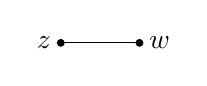
\begin{tikzpicture}
        \fill (0,0) circle (0.05) node[left] {\(z\)};
        \fill (1,0) circle (0.05) node[right] {\(w\)};
        \draw (0,0) -- (1,0);
    \end{tikzpicture}
\end{figure}
This represents creation of a particle at \(w\) and annihilation at \(z\). For \(n=4\), there are three such processes for indistinguisable particles:
\begin{figure}[H]
    \centering
    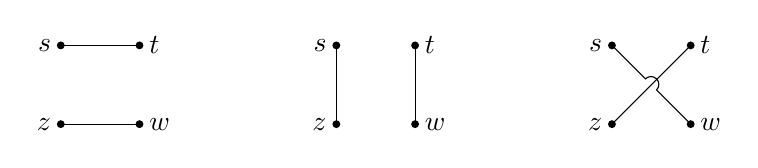
\begin{tikzpicture}
        \begin{scope}
            \fill (0,0) circle (0.05) node[left] {\(z\)};
            \fill (1,0) circle (0.05) node[right] {\(w\)};
            \fill (0,1) circle (0.05) node[left] {\(s\)};
            \fill (1,1) circle (0.05) node[right] {\(t\)};
            \draw (0,0) -- (1,0);
            \draw (0,1) -- (1,1);
        \end{scope}
        \begin{scope}[shift={(3.5,0)}]
            \fill (0,0) circle (0.05) node[left] {\(z\)};
            \fill (1,0) circle (0.05) node[right] {\(w\)};
            \fill (0,1) circle (0.05) node[left] {\(s\)};
            \fill (1,1) circle (0.05) node[right] {\(t\)};
            \draw (0,0) -- (0,1);
            \draw (1,0) -- (1,1);
        \end{scope}
        \begin{scope}[shift={(7,0)}]
            \fill (0,0) circle (0.05) node[left] {\(z\)};
            \fill (1,0) circle (0.05) node[right] {\(w\)};
            \fill (0,1) circle (0.05) node[left] {\(s\)};
            \fill (1,1) circle (0.05) node[right] {\(t\)};
            \draw (0,0) -- (1,1);
            \draw (0,1) -- (0.425,0.575) arc (135:-45:0.1) -- (1,0);
        \end{scope}
    \end{tikzpicture}
\end{figure}
The fact that the amplitudes are the same for each pair is a reflection of Bose statistics.

Similarly for \(n\) particles, one gets the sum of all ways of joining pairs of points.

\subsection{Interaction}
The only allowed interaction terms (for reasons) are of the form \(\mathcal{L}_{\mathrm{I}} = -\frac{\lambda\phi^4}{4!}\) or \(+\frac{g\phi^3}{3!}\). The full Lagrangian is
\begin{equation}
    \mathcal{L} = -\frac{1}{2}(\partial\phi)^2-\frac{1}{2}m^2\phi^2 + \mathcal{L}_{\mathrm{I}} + iJ\phi.
\end{equation}
The resultant equations of motion (setting \(J=0\)) are
\begin{equation}
    (\dalembertian - m^2)\phi=\frac{g\phi^2}{2} \,\text{or}\, -\frac{\lambda\phi^3}{6}.
\end{equation}
These are non-linear equations for which general analytic solutions do not exist. Even if we could solve these equations, the solutions could not be linearly superposed. Therefore we will treat these cases with perturbation theory, expanding in powers of \(g\) or \(\lambda\).

We have
\begin{equation}
    Z_1(J) = \int\Dd{\phi}e^{i\int\mathcal{L}_0+\mathcal{L}_{\mathrm{I}}\dd[4]{x}} = \int\Dd{\phi}e^{i\int\mathcal{L}_{\mathrm{I}}\dd[4]{x}}e^{i\int\mathcal{L}_0\dd[4]{x}}.
\end{equation}
Note that \(-\fdv{J(x)}\) acting on \(e^{i\int\mathcal{L}_0}\dd[4]{x}\) gives \(\phi(x)e^{i\int\mathcal{L}_0}\dd[4]{x}\). Hence we can replace \(e^{i\int\mathcal{L}_I[\phi(x)]}\dd[4]{x}\) by \(e^{i\int\mathcal{L}_I\left(-\fdv{J(x)}\right)}\dd[4]{x}\) in the above expression. We obtain
\begin{equation}
    Z_1(J) = \int\Dd{\phi}e^{i\int\mathcal{L}_{\mathrm{I}}\left(-\fdv{J(x)}\right)\dd[4]{x}}e^{i\int\mathcal{L}_0\dd[4]{x}} = e^{i\int\mathcal{L}_I\left(-\fdv{J(x)}\right)}\dd[4]{x} Z_0(J).
\end{equation}
Thus we have (up to normalisation)
\begin{equation}
    Z_1(J)\sim \exp(i\int\mathcal{L}_I\left(-\fdv{J(x)}\right)) \underbrace{\exp(\frac{1}{2}\int\dd[4]{x}\dd[4]{y}J(x)\Delta_F(x-y)J(y))}_{\sim Z_0}.
    \tag{\(*\)}
    \label{interaction}
\end{equation}

\subsection{\texorpdfstring{$\phi^3$}{Phi-cubed} theory}
Let's set \(\mathcal{L}_{\mathrm{I}} = \frac{g\phi^3}{3!}\) and evaluate \eqref{interaction}. We have
\begin{equation}
    Z_1(J) = \sum^\infty_{V=0}\left[\int\dd[4]{x}\left(-\fdv{J(x)}\right)^3\right]^V\frac{g^Vi^V}{V!(3!)^V} \times \sum^\infty_{P=0}\left[\int\dd[4]{y}\dd[4]{z}J(y)\Delta_F(y-z)J(z)\right]^P \frac{1}{P!}\frac{1}{2^P}.
\end{equation}
Note that this is an asymptotic series, but not a convergent one. Each term in the series will be \(\sim g^V J^E \Delta_F^P\), where \(E = 2P-3V\). We organise the expansion in powers of \(E\) and \(V\).

The diagrammatic analogy continues here. We will start with the diagrams, and then explain how they relate to the series expansion for \(Z_1(J)\). For each \(E,V,P\), we draw all possible graphs with \(V\) vertices, \(P\) internal lines, and \(E\) external lines. Internal vertices must be trivalent.

At \(E=0,V=2,P=3\) we have:
\begin{figure}[H]
    \centering
    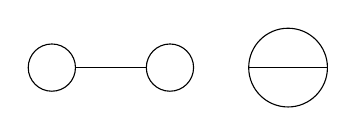
\begin{tikzpicture}
        \draw (0,0) circle (0.3);
        \draw (1.5,0) circle (0.3);
        \draw (0.3,0) -- (1.2,0);

        \draw (3,0) circle (0.5);
        \draw (2.5,0) -- (3.5,0);
    \end{tikzpicture}
\end{figure}
\(E=0,V=4,P=6\):
\begin{figure}[H]
    \centering
    \begin{tikzpicture}
        \draw (0,0) circle (0.3);
        \draw (1.5,0) circle (0.3);
        \draw (3.0,0) circle (0.3);
        \draw (0.3,0) -- (1.2,0);
        \draw (1.8,0) -- (2.7,0);

        \draw (4.5,0) circle (0.3);
        \draw (6.2,0) circle (0.5);
        \draw (4.8,0) -- (5.7,0);
        \draw (6.2,0.5) -- (6.2,-0.5);

        \draw (8.65,0) circle (0.75);
        \draw[fill=white] (7.9,0) circle (0.3);
        \draw[fill=white] (9.4,0) circle (0.3);

        \begin{scope}[shift={(2.5,-2.5)}]
            \begin{scope}[rotate=120]
                \draw (0,0) -- (0,0.4);
                \draw (0,0.7) circle (0.3);
            \end{scope}
            \begin{scope}[rotate=240]
                \draw (0,0) -- (0,0.4);
                \draw (0,0.7) circle (0.3);
            \end{scope}
            \begin{scope}
                \draw (0,0) -- (0,0.4);
                \draw (0,0.7) circle (0.3);
            \end{scope}
        \end{scope}

        \begin{scope}[shift={(6.5,-2.5)}]
            \draw (0,0) circle (0.75);
            \foreach \x in {0,120,240} {\draw (0,0) -- ({0.75*cos(\x)},{0.75*sin(\x)});}
        \end{scope}
    \end{tikzpicture}
\end{figure}
The above are all \emph{connected} diagrams. They are also all \emph{vacuum} diagrams, i.e.\ they have no left over powers of \(J\) and hence no external lines. When we have \(P\) non-zero, we get non-vacuum diagrams.

\(E=1,V=1,P=2\):
\begin{figure}[H]
    \centering
    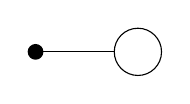
\begin{tikzpicture}
        \fill (0,0) circle (0.1);
        \draw (0,0) -- (1,0);
        \draw (1.3,0) circle (0.3);
    \end{tikzpicture}
\end{figure}
This type of diagram is known as a \emph{tadpole} diagram, for hopefully obvious reasons.

\(E=1,V=3,P=5\):
\begin{figure}[H]
    \centering
    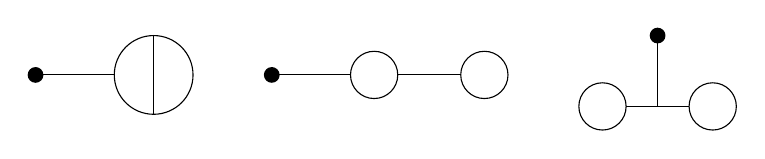
\begin{tikzpicture}
        \fill (0,0) circle (0.1);
        \draw (0,0) -- (1,0);
        \draw (1.5,0) circle (0.5);
        \draw (1.5,0.5) -- (1.5,-0.5);

        \fill (3,0) circle (0.1);
        \draw (3,0) -- (4,0);
        \draw (4.6,0) -- (5.4,0);
        \draw (4.3,0) circle (0.3);
        \draw (5.7,0) circle (0.3);

        \draw (7.2,-0.4) circle (0.3);
        \draw (8.6,-0.4) circle (0.3);
        \draw (7.5,-0.4) -- (8.3,-0.4);
        \draw (7.9,-0.4) -- (7.9,0.5);
        \fill (7.9,0.5) circle (0.1);
    \end{tikzpicture}
\end{figure}

\(E=2,V=0,P=1\):
\begin{figure}[H]
    \centering
    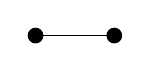
\begin{tikzpicture}
        \fill (0,0) circle (0.1);
        \fill (1,0) circle (0.1);
        \draw (0,0) -- (1,0);
    \end{tikzpicture}
\end{figure}

\(E=2,V=2,P=4\):
\begin{figure}[H]
    \centering
    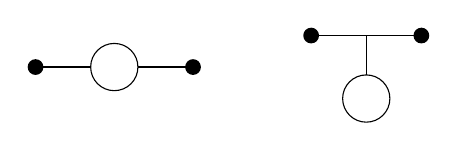
\begin{tikzpicture}
        \fill (0,0) circle (0.1);
        \fill (2,0) circle (0.1);
        \draw (0,0) -- (2,0);
        \draw[fill=white] (1,0) circle (0.3);

        \fill (3.5,0.4) circle (0.1);
        \fill (4.9,0.4) circle (0.1);
        \draw (3.5,0.4) -- (4.9,0.4);
        \draw (4.2,0.4) -- (4.2,-0.1);
        \draw (4.2,-0.4) circle (0.3);
    \end{tikzpicture}
\end{figure}

\(E=3,V=1,P=3\):
\begin{figure}[H]
    \centering
    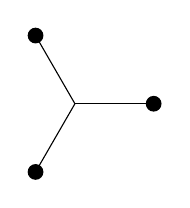
\begin{tikzpicture}
        \foreach \x in {0,120,240} {
            \draw (0,0) -- ({cos(\x)},{sin(\x)});
            \fill ({cos(\x)},{sin(\x)}) circle (0.1);
        }
    \end{tikzpicture}
\end{figure}
This particular diagram is known as the \emph{vertex function}.

\(E=3,V=3,P=6\):
\begin{figure}[H]
    \centering
    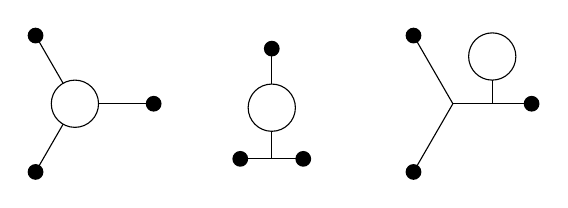
\begin{tikzpicture}
        \foreach \x in {0,120,240} {
            \draw (0,0) -- ({cos(\x)},{sin(\x)});
            \fill ({cos(\x)},{sin(\x)}) circle (0.1);
        }
        \draw[fill=white] (0,0) circle (0.3);

        \draw (2.5,0.7) -- (2.5,-0.7);
        \draw (2.1,-0.7) -- (2.9,-0.7);
        \draw[fill=white] (2.5,-0.05) circle (0.3);
        \fill (2.5,0.7) circle (0.1);
        \fill (2.1,-0.7) circle (0.1);
        \fill (2.9,-0.7) circle (0.1);

        \foreach \x in {0,120,240} {
            \draw (4.8,0) -- ({4.8+cos(\x)},{sin(\x)});
            \fill ({4.8+cos(\x)},{sin(\x)}) circle (0.1);
        }
        \draw (5.3,0.6) circle (0.3);
        \draw (5.3,0) -- (5.3,0.3);
    \end{tikzpicture}
\end{figure}

Each of these diagrams is associated with a number, which we construct in the following way. We give each vertex and internal line a variable name (e.g.\ \(x\)). We add a factor of \(\Delta_F(x-y)\) for each internal line, where \(x\) and \(y\) are the vertices it connects. We put in an integral \(\int\dd[4]{x}g\) for each vertex and \(\int\dd[4]{x}J(x)\) for each external line. We multiply by a phase factor \(i^{P-2V}\), and finally divide by a ``symmetry factor'' \(S\), which we will explain shortly. This then gives the contribution to \(Z_1(J)\) represented by each diagram.

The symmetry factor is relatively simple to calculate. Since we have attached labels to vertices and external lines, we have actually overcounted, and must take away these factors. If there were absolutely no symmetry in the diagram, we would have the following. Permutations of attaching lines at a fixed vertex gives a \(3!\) which cancels the \(\frac{1}{3!}\) in \(\frac{g\phi^3}{3!}\). There are 2 arrangements of each internal line, depending on the labelling of its ends, and permutations of the lines give \(P!\) ways of arranging the propagators, so these cancel the factor of \(\frac{1}{P!2^P}\). \emph{However}, there is often a certain amount of symmetry in the diagrams, so there are actually fewer permutations than we have accounted for. Hence, we divide by a number that represents how distant the diagrams are from perfect asymmetry. Some examples:
\begin{table}[H]
    \centering
    \hfuzz=18pt 
    \begin{tabular}{ccl}
        \raisebox{-.35\height}{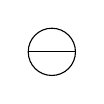
\begin{tikzpicture}
            \draw (0,0) circle (0.3);
            \draw (-0.3,0) -- (0.3,0);
        \end{tikzpicture}} & \(S=3!\) & \text{because propagators are indistinguishable}\\\\
        \raisebox{-.35\height}{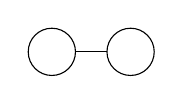
\begin{tikzpicture}
            \draw (0,0) circle (0.3);
            \draw (1,0) circle (0.3);
            \draw (0.3,0) -- (0.7,0);
        \end{tikzpicture}} & \(S=8\) & \text{because vertices are indistinguishable and loops can be oriented 2 ways}\\\\
        \raisebox{-.35\height}{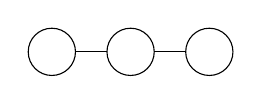
\begin{tikzpicture}
            \draw (0,0) circle (0.3);
            \draw (1,0) circle (0.3);
            \draw (2,0) circle (0.3);
            \draw (0.3,0) -- (0.7,0);
            \draw (1.3,0) -- (1.7,0);
        \end{tikzpicture}} & \(S=2^4\)\\\\
        \raisebox{-.35\height}{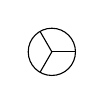
\begin{tikzpicture}
            \draw (0,0) circle (0.3);
            \foreach \x in {0,120,240} {\draw (0,0) -- ({0.3*cos(\x)},{0.3*sin(\x)});}
        \end{tikzpicture}} & \(S=4!\)
    \end{tabular}
\end{table}

These diagrams are a way of identifying to \(Z_1(g,J)\) of order \(g^VJ^E\). Each propagator factor has two ends, each vertex has three propagators attached to it, and each \(J\) must have a single end, so \(3V+E=2P\).

All of these diagrams have been connected, but the expansion of \(Z_1(g,J)\) contains disconnected diagrams. These correspond to processes that factorise into a number of disjoint processes. For example, with \(E=0,V=4,P=6\), we might have:
\begin{figure}[H]
    \centering
    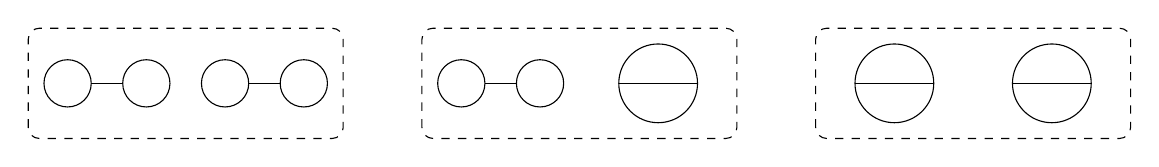
\begin{tikzpicture}
        \begin{scope}
            \draw (0,0) circle (0.3);
            \draw (1,0) circle (0.3);
            \draw (0.3,0) -- (0.7,0);

            \draw (2,0) circle (0.3);
            \draw (3,0) circle (0.3);
            \draw (2.3,0) -- (2.7,0);
            \draw[rounded corners,dashed] (-0.5,-0.7) rectangle (3.5,0.7);
        \end{scope}
        \begin{scope}[shift={(5,0)}]
            \draw (0,0) circle (0.3);
            \draw (1,0) circle (0.3);
            \draw (0.3,0) -- (0.7,0);

            \draw (2.5,0) circle (0.5);
            \draw (2,0) -- (3,0);
            \draw[rounded corners,dashed] (-0.5,-0.7) rectangle (3.5,0.7);
        \end{scope}
        \begin{scope}[shift={(10,0)}]
            \draw (0.5,0) circle (0.5);
            \draw (0,0) -- (1,0);

            \draw (2.5,0) circle (0.5);
            \draw (2,0) -- (3,0);
            \draw[rounded corners,dashed] (-0.5,-0.7) rectangle (3.5,0.7);
        \end{scope}
    \end{tikzpicture}
\end{figure}
We can write
\begin{equation}
    Z_1(J) = \sum_{\substack{\text{all distinct}\\\text{diagrams}}} \prod_I \frac{1}{N_I!}C_I^{N_I},
\end{equation}
where \(C_I\) refers to the contribution of a particular connected diagram, and \(N_I\) refers to the number of times it appears. We can swap any two connected components and the whole diagram is not affected, so \(N_I!\) is a symmetry factor here. The sum is over all possible combinations of \(N_I\), so we have
\begin{equation}
    Z_1(J) = \prod_I\sum^\infty_{N=0}\frac{1}{N!}C_I^N = \prod_I\exp C_I = \exp(\sum_IC_I) = \exp(iW_1(J,g)),
\end{equation}
where \(iW_1\) is the sum of amplitudes of connected diagrams. Thus there is no need to find contributions from disconnected diagrams. All one need do is to exponentiate the sum of connected diagrams. Using \(Z_1=e^{iW_1}\), we have
\begin{equation}
    \mel{0}{T\phi(w)\phi(z)}{0} 
    = \left.\fdv{J(x_1)}\fdv{J(x_2)}Z_1(J)\right|_{J=0}
    = i\left.\fdv{J(x_1)}\fdv{J(x_2)}W_1\right|_{J=0},
\end{equation}
and we can also calculate
\begin{equation}
    \mel{0}{T\phi(x_1)\phi(x_2)\phi(x_3)\phi(x_4)}{0}
    = \left[i\delta_1\delta_2\delta_3\delta_4W 
        - \delta_1\delta_2W\delta_3\delta_4W
        - \delta_1\delta_3W\delta_2\delta_4W
    - \delta_1\delta_4W\delta_2\delta_3W\right].
\end{equation}

Consider now the amplitude for four particle interactions to order \(g^2\), with two particles in the past and two particles in the future. If we label each external line (particle), then there are three possible diagrams:
\begin{figure}[H]
    \centering
    \begin{tikzpicture}
        \begin{scope}
            \draw (0,0) -- (-1,1) node[above left] {\(1\)};
            \draw (0,0) -- (-1,-1) node[below left] {\(2\)};
            \draw (2,0) -- (3,1) node[above right] {\(1'\)};
            \draw (2,0) -- (3,-1) node[below right] {\(2'\)};
            \draw (0,0) -- (2,0);
            \draw[very thick,->] (-0.51,0.51) -- (-0.5,0.5) node[above right] {\(k_1\)};
            \draw[very thick,->] (-0.51,-0.51) -- (-0.5,-0.5) node[above left] {\(k_2\)};
            \draw[very thick,->] (2.49,0.49) -- (2.5,0.5) node[above left] {\(k_1'\)};
            \draw[very thick,->] (2.49,-0.49) -- (2.5,-0.5) node[above right] {\(k_2'\)};
            \draw[very thick,->] (0.99,0) -- (1,0) node[below]{\(k=k_1+k_2\)};
        \end{scope}
        \begin{scope}[shift={(7,-1)},rotate=90]
            \draw (0,0) -- (-1,1) node[below left] {\(2\)};
            \draw (0,0) -- (-1,-1) node[below right] {\(2'\)};
            \draw (2,0) -- (3,1) node[above left] {\(1\)};
            \draw (2,0) -- (3,-1) node[above right] {\(1'\)};
            \draw (0,0) -- (2,0);
            \draw[very thick,->] (-0.51,0.51) -- (-0.5,0.5) node[above left] {\(k_2\)};
            \draw[very thick,<-] (-0.51,-0.51) -- (-0.5,-0.5) node[below left] {\(k_2'\)};
            \draw[very thick,<-] (2.49,0.49) -- (2.5,0.5) node[below left] {\(k_1\)};
            \draw[very thick,->] (2.49,-0.49) -- (2.5,-0.5) node[above left] {\(k_1'\)};
            \draw[very thick,<-] (0.99,0) -- (1,0) node[right]{\(k=k_1-k_1'\)};
        \end{scope}
        \begin{scope}[shift={(3,-4.5)}]
            \draw (-1,1) node[above left] {\(1\)} -- (3,-1) node[below right] {\(2'\)};
            \draw (-1,-1) node[below left] {\(2\)} -- (0.9,-0.1) arc (210:30:0.13) -- (3,1) node[above right] {\(1'\)};
            \draw (0.2,0.4) -- (0.2,-0.43);

            \draw[very thick,->] (-0.4, 0.7) -- (-0.38,0.69) node[above right] {\(k_1\)};
            \draw[very thick,->] (-0.4, -0.7) -- (-0.38,-0.69) node[below right] {\(k_2\)};
            \draw[very thick,->] (2,0.5) -- (2.02,0.51) node[above left] {\(k_1'\)};
            \draw[very thick,->] (2,-0.5) -- (2.02,-0.51) node[below left] {\(k_2'\)};
            \draw[very thick,<-] (0.2,0) -- (0.2,0.01) node[left] {\(k=k_1-k_2'\)};
        \end{scope}
    \end{tikzpicture}
\end{figure}
Rather than treat these amplitudes as functions of spacetime, we instead look at their Fourier transforms and label the particle states by their momenta. To do this we must translate the computational rules into momentum space. In coordinate space one has to integrate over all position in spacetime of each vertex. We have
\begin{align}
    \braket{f}{i} &= ig^2\int\frac{\dd[4]{k}}{(2\pi)^4}\frac{1}{k^2+m^2-i\epsilon} \\
                  &\qquad \big[ (2\pi)^4\delta^4(k_1+k_2-k)(2\pi)^4\delta^4(k_1'+k_2'-k) \\
                  &\qquad\qquad + (2\pi)^4\delta^4(k_1-k_1'-k)(2\pi)^4\delta^4(k_2-k_2'-k) \\
                  &\qquad\qquad + (2\pi)^4\delta^4(k_1-k_2'-k)(2\pi)^4\delta^4(k_1'-k_2-k) \big] \\
                  &= ig^2(2\pi)^4\underbrace{\delta^4(k_1+k_2-k_1'-k_2')}_{\text{momentum conservation}} T,
\end{align}
where
\begin{equation}
    T = \frac{1}{(k_1+k_2)^2+m^2-i\epsilon} + \frac{1}{(k_1-k_1')^2+m^2-i\epsilon} + \frac{1}{(k_1-k_2')^2+m^2-i\epsilon}
\end{equation}
is the \emph{transfer matrix} for this process. This is tree-level scattering (no loops).

The rules for calculating these amplitudes with diagrams for a given theory are known as its \emph{Feynman rules}. To summarise, the momentum space Feynman rules are:
\begin{enumerate}
    \item Draw all diagrams to the appropriate order.
    \item Label each ingoing and outgoing line with its momentum.
    \item Conserve momentum at each vertex, so add a factor \((2\pi)^4\delta^{(4)}(k_1+k_2+k_3)\).
    \item For each internal line, add a factor of the Feynman propagator \(\frac{-i}{k^2+m^2-i\epsilon}\).
    \item For each vertex, add a factor of \(ig\).
    \item For each undetermined momentum, integrate \(\int\frac{\dd[4]{k}}{(2\pi)^4}\).
    \item Divide by the symmetry factor.
    \item Add all terms to get the transfer matrix.
\end{enumerate}

\subsection{\texorpdfstring{$\phi^4$}{Phi to the fourth} theory}
If we have \(\mathcal{L}_{\mathrm{I}} = -\frac{\lambda\phi^4}{4!}\), then the Feynman rules are exactly the same, except vertices must now be 4-valent, and come with a factor of \(-i\lambda\). Let's calculate the transfer matrix for the scattering from two particles to two particles, to order \(\lambda^2\). We have the following diagrams:
\begin{figure}[H]
    \centering
    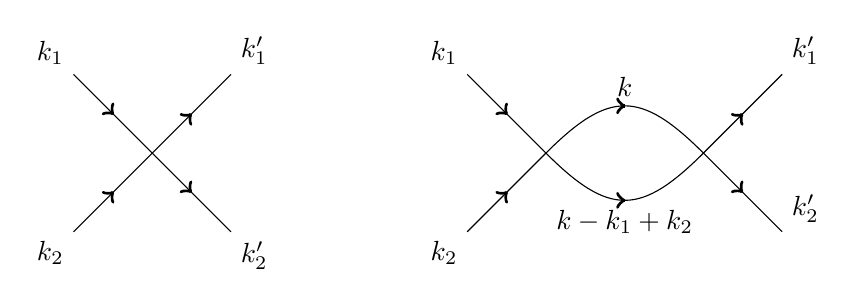
\begin{tikzpicture}
        \draw (-1,1) node[above left] {\(k_1\)} -- (1,-1) node[below right] {\(k_2'\)};
        \draw (-1,-1) node[below left] {\(k_2\)} -- (1,1) node[above right] {\(k_1'\)};
        \draw[very thick,->] (-0.5,0.5) -- (-0.49,0.49);
        \draw[very thick,->] (-0.5,-0.5) -- (-0.49,-0.49);
        \draw[very thick,<-] (0.5,-0.5) -- (0.49,-0.49);
        \draw[very thick,<-] (0.5,0.5) -- (0.49,0.49);

        \begin{scope}[shift={(5,0)}]
            \draw (-1,1) node[above left] {\(k_1\)} -- (0,0) .. controls (0.8,-0.8) and (1.2,-0.8) .. (2,0) node[midway,below] {\(k-k_1+k_2\)} -- (3,1) node[above right] {\(k_1'\)};
            \draw (-1,-1) node[below left] {\(k_2\)} -- (0,0) .. controls (0.8,0.8) and (1.2,0.8) .. (2,0) node[midway,above] {\(k\)} -- (3,-1) node[above right] {\(k_2'\)};
            \draw[very thick,->] (-0.5,0.5) -- (-0.49,0.49);
            \draw[very thick,->] (-0.5,-0.5) -- (-0.49,-0.49);
            \draw[very thick,<-] (2.5,0.5) -- (2.49,0.49);
            \draw[very thick,<-] (2.5,-0.5) -- (2.49,-0.49);
            \draw[very thick,->] (1,0.6) -- (1.01,0.6);
            \draw[very thick,->] (1,-0.6) -- (1.01,-0.6);
        \end{scope}
    \end{tikzpicture}
\end{figure}
We ignore other diagrams for now. Using the Feynman rules, this translates to
\begin{equation}
    iT = \lambda + \frac{-\lambda^2}{2}\int\frac{\dd[4]{k}}{(2\pi)^4}\frac{-i}{k^2+m^2-i\epsilon}\frac{-i}{(k-l)^2+m^2-i\epsilon},
\end{equation}
where \(l = k_1+k_2\). Set \(m^2=0\) (so a massless field), The \(O(\lambda^2)\) part
\begin{equation}
    f(s=l^2) = \frac{i\lambda^2}{2}\int\frac{\dd[4]{k}}{(2\pi)^4}\frac{1}{k^2}\frac{1}{(k-l)^2}
\end{equation}
is a divergent integral, so we will need to regularise it in some fashion.

A commonly used identity for transforming integrals of this form is the so-called ``Feynman parameter formula'':
\begin{equation}
    \frac{1}{xy} = \int_0^1\dd{\alpha}\frac{1}{(\alpha x + (1-\alpha) y)^2}
\end{equation}
Using this with \(x=(k-l)^2\) and \(y=k^2\), we have
\begin{align}
    f(s) &= \frac{i\lambda^2}{2}\int\frac{\dd[4]{k}}{(2\pi)^4}\int_0^1\dd{\alpha}\frac{1}{[\alpha(k-l)^2+(1-\alpha)k^2]^2} \\
         &= \frac{i\lambda^2}{2}\int\frac{\dd[4]{k}}{(2\pi)^4}\int_0^1\dd{\alpha}\frac{1}{[k^2 - 2\alpha k\vdot l + \alpha l^2]^2} \\
         &= \frac{i\lambda^2}{2}\int\frac{\dd[4]{k}}{(2\pi)^4}\int_0^1\dd{\alpha}\frac{1}{[(k-\alpha l)^2 + \alpha(1-\alpha)l^2]^2} 
    \intertext{(now shift the origin of the momentum integral)}
         &= \frac{i\lambda^2}{2}\int\frac{\dd[4]{k}}{(2\pi)^4}\int_0^1\dd{\alpha}\frac{1}{[k^2 + \alpha(1-\alpha)l^2]^2}.
\end{align}

We will use \emph{Pauli-Villars regularisation}: we introduce a cut-off for large momenta. Note that \(\int\dd[4]{k}\) is an integral over all momenta, with \(\dd[4]{k}=\dd[3]{k}\dd{k^0}\), and \(k^2 = -{k^0}^2+\vb{k}^2\). The (ignored here) factors of \(i\epsilon\) amount to saying that the integration over \(k^0\) is along the imaginary axis. Hence we can rotate the \(k^0\) contour, setting \(k^0\to ik^0\). Now we have \(k^2={k^0}^2+\vb{k}^2\). We get
\begin{equation}
    f(s) = \frac{\lambda^2}{2}\int\frac{\dd[4]{k}}{(2\pi)^4}\int_0^1\dd{\alpha}\frac{1}{[k^2 + \alpha(1-\alpha)l^2]^2}
\end{equation}
where \(k\) is now in real space, and \(k^2\) is Euclidean. Introduce polar coordinates in momentum space, so that \(\dd[4]{k}\to k^3\dd{k}\dd{\Omega_k}\), where \(\dd{\Omega_k}\) is the volume element of the unit 3-sphere. Nothing depends on the direction of \(k\), so \(\int\dd{\Omega_k}=2\pi^2\). Hence we have
\begin{equation}
    f(s) = \frac{\lambda^2}{16\pi^2}\int^\Lambda_0 k^3\dd{k} \int^1_0 \dd{\alpha}\frac{1}{[k^2+\alpha(1-\alpha)l^2]^2}.
\end{equation}
We integrate only up to \(|k|=\Lambda\) --- this is the momentum cut-off of the Pauli-Villars regularisation. We write \(A=\sqrt{\alpha(1-\alpha)l^2}\). We have
\begin{align}
    f(s) &= \frac{\lambda^2}{16\pi^2}\int^\Lambda_0 k^3\dd{k}\int^1_0\dd{\alpha}\frac{1}{[k^2+A^2]^2}
    \intertext{(now rescale \(k \to z=k/A\))}
    &= \frac{\lambda^2}{16\pi^2}\int^1_0\dd{\alpha}\int^{\Lambda/A}_0 z^3\dd{z} \frac{1}{(z^2+1)^2}
    \intertext{(set \(z=\sinh\theta\))}
    &= \frac{\lambda^2}{16\pi^2}\int^1_0\dd{\alpha}\int^{\Lambda/A}_0\frac{\sinh^3\theta\cosh\theta\dd{\theta}}{\cosh^4\theta} \\
    &= \frac{\lambda^2}{16\pi^2}\int^1_0\dd{\alpha}\int^{\Lambda/A}_0\tanh^3\theta\dd{\theta} \\
    &= \frac{\lambda^2}{16\pi^2}\int^1_0\dd{\alpha} \left[\log\cosh\theta-\frac{1}{2}\tanh^2\theta\right]^{z=\Lambda/A}_0 \\
    &= \frac{\lambda^2}{16\pi^2}\int^1_0\dd{\alpha} \left[\frac{1}{2}\log(1+z^2) - \frac{z^2}{2(1+z^2)}\right]^{\Lambda/A}_0 \\
    &= \frac{\lambda^2}{16\pi^2}\int^1_0\dd{\alpha} \left[\frac{1}{2}\log(1+\frac{\Lambda^2}{A^2}) - \frac{\Lambda^2/A^2}{2(1+\Lambda^2/A^2)}\right] \\
    &= \frac{\lambda^2}{32\pi^2}\int^1_0\dd{\alpha}\left[\log(\frac{\Lambda^2}{A^2})+\log(1+\frac{A^2}{\Lambda^2}) - \frac{1}{1+A^2/\Lambda^2}\right]
    \intertext{(now assume the cutoff is large, i.e.\ \(\Lambda^2\gg A^2\))}
    &\approx \frac{\lambda^2}{32\pi^2}\int^1_0\dd{\alpha}\left[\log(\Lambda^2) - \log(l^2\alpha(1-\alpha)) - 1\right] \\
    &= \frac{\lambda^2}{32\pi^2}\left[\alpha\log\frac{\Lambda^2}{l^2} - \alpha\log\alpha+(1-\alpha)\log(1-\alpha) - 1 - \alpha\right]^1_0 \\
    &= \frac{\lambda^2}{32\pi^2}\log\frac{\Lambda^2}{l^2} + \text{constant}.
\end{align}
Observe that although the regularised amplitude is finite, we really want to take the limit as \(\Lambda to \infty\), since we are supposed to integrate over all momenta.

So the amplitude for 2 particles to go to 2 particles, for the case \(s=l^2\), is given by
\begin{equation}
    iT(s) = \lambda + \frac{\lambda^2}{32\pi^2}\log\frac{\Lambda^2}{s} + (\text{constant}).
\end{equation}
The input into the theory is a coupling constant \(\lambda\), and an incoming energy parametrised by \(s\), but \(T\) depends on \(\Lambda\), so this looks like it might be nonsense. To get around this, we write \(\lambda_R=T(s_0)\): this is the \emph{renormalised} coupling constant. In an actual experiment, we measure the amplitude at some energy. Consider the amplitude \(T(s_0)\) and compare it to \(T(s_1)\). We have
\begin{equation}
    T(s_1)-T(s_0) = \frac{\lambda^2}{32\pi^2}\log(\frac{s_1}{s_0}),
\end{equation}
so the difference between the amplitudes is finite. We have
\begin{equation}
    \lambda_R = \lambda + \frac{\lambda^2}{32\pi^2}\log\frac{\Lambda^2}{s_0}.
\end{equation}
Inverting this series, we obtain
\begin{equation}
    \lambda \approx \lambda_R - \frac{\lambda_R^2}{32\pi^2}\log\frac{\Lambda^2}{s_0}.
\end{equation}
Hence we can find
\begin{align}
    T(s_1) &= \lambda + \frac{\lambda^2}{32\pi^2}\log\frac{\Lambda^2}{s_1} \\
           &= \lambda_R - \frac{\lambda_R^2}{32\pi^2}\log\frac{\Lambda^2}{s_0} + \frac{\lambda_R^2}{32\pi^2}\log\frac{\Lambda^2}{s_1} + O(\lambda_R^3) \\
           &\approx \lambda_R - \frac{\lambda_R^2}{32\pi^2}\log\frac{s_1}{s_0}.
\end{align}
We choose \(\lambda_R\) to be finite. Since \(\Lambda \to \infty\), this means we must have \(\lambda \to \infty\). So the output is: given amplitudes at some energy scale, you can calculate amplitudes at another energy scale.

The justification of this method is that it (sometimes) works.

There are only two other things that can be renormalised: the masses of particles, and the overall normalisation of the fields (\emph{wavefunction renormalisation}).

The 1-loop diagrams that we did not consider above only add a constant for fixed external momenta to the amplitudes, so they do not change differences in amplitudes.

\subsection{Higher loops}
There are contributions to the amplitude with more loops:
\begin{figure}[H]
    \centering
    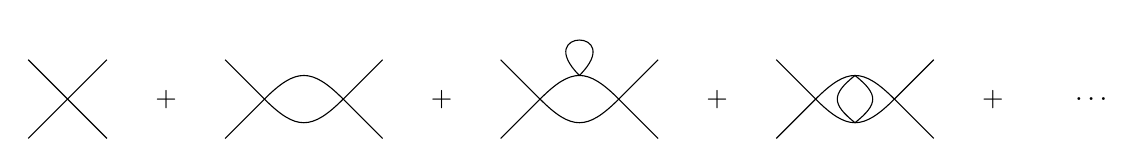
\begin{tikzpicture}
        \draw (0,0) -- (1,1);
        \draw (1,0) -- (0,1);

        \node at (1.75,0.5) {\(+\)};

        \draw (2.5,0) -- (3,0.5) .. controls (3.4,0.9) and (3.6,0.9) .. (4,0.5) -- (4.5,0);
        \draw (2.5,1) -- (3,0.5) .. controls (3.4,0.1) and (3.6,0.1) .. (4,0.5) -- (4.5,1);

        \node at (5.25,0.5) {\(+\)};

        \begin{scope}[shift={(3.5,0)}]
            \draw (2.5,0) -- (3,0.5) .. controls (3.4,0.9) and (3.6,0.9) .. (4,0.5) -- (4.5,0);
            \draw (2.5,1) -- (3,0.5) .. controls (3.4,0.1) and (3.6,0.1) .. (4,0.5) -- (4.5,1);
            \begin{scope}[shift={(3.5,0.8)},scale=0.6]
                \draw (0,0) .. controls (1,1) and (-1,1) .. (0,0);
            \end{scope}
        \end{scope}

        \node at (8.75,0.5) {\(+\)};
        
        \begin{scope}[shift={(7,0)}]
            \draw (2.5,0) -- (3,0.5) .. controls (3.4,0.9) and (3.6,0.9) .. (4,0.5) -- (4.5,0);
            \draw (2.5,1) -- (3,0.5) .. controls (3.4,0.1) and (3.6,0.1) .. (4,0.5) -- (4.5,1);
            \begin{scope}[shift={(3.5,0.5)},scale=0.3]
                \draw (0,-1) .. controls (1,-0.2) and (1,0.2) .. (0,1);
                \draw (0,-1) .. controls (-1,-0.2) and (-1,0.2) .. (0,1);
            \end{scope}
        \end{scope}

        \node at (12.25,0.5) {\(+\)};
        \node at (13.5,0.5) {\(\dots\)};
    \end{tikzpicture}
\end{figure}

If we include powers of \(\hbar\), then an \(L\)-loop diagram contributes a term to the amplitude of order \(\hbar^L\). Note that the amplitude as a power series expansion in powers of the coupling constant is usually asymptotic. If we write \(T=\sum\lambda^nT_n\), then this series becomes useless when \(n\sim\frac{1}{\lambda}\).

Suppose we have a Feynman diagram with \(\phi^N\) interactions that has \(P\) propagators, \(E\) external lines, \(V\) vertices, and \(L\) loops (i.e.\ the number of undetermined momenta in the diagram). Since each propagator has 2 ends, we can write \(E+2P=NV\). Also, the momenta are constrained by conservation at each vertex and for the overall diagram, so the number of undetermined momenta is \(L=P-V+1\). If we were to evaluate the Feynman diagram, with a momentum cutoff \(\Lambda\), we would get something that looked like
\begin{equation}
    \underbrace{(\text{momentum})^{4L}}_{\substack{\dd[4]{p}\\\text{for loops}}} \underbrace{\frac{1}{(\text{momentum})^{2P}}}_{\text{propagators}} \sim \Lambda^{4L-2P}.
\end{equation}
We call this exponent \(D=4L-2P\) the primitive degree of divergence (if \(D\ge0\)). We have \(D = 4(P-V+1)-2P = 2P-4V-4\). For \(D=0\), as \(\Lambda\to\infty\) we encounter a logarithmic divergence \(\log\Lambda^2\), as in the previous section. For higher \(D\) we get faster divergences. For example \(D=2\) leads to a quadratic divergence. If \(D<0\), then the contribution to the amplitude vanishes as \(\Lambda \to \infty\).

In a general diagram, \(D = 2P-4V+4 = NV-4V+4-E = V(N-4)+4-E\). So from this we can more or less see that arbitrary interactions are impossible. For \(N \le 4\), there are only a finite number of different types of divergence: we say this theory is \emph{renormalisable}. For \(N \ge 5\), there are an infinite number of types of divergence. Such a theory is nonrenormalisable, and do not exist as QFTs.

\subsection{Free fermions}
If we add a source term to the Dirac action, we have
\begin{equation}
    S = \int\dd[4]{x} \overline{\psi}(i\gamma^a\partial_a - m)\psi + \overline{\eta}\psi + \overline{\psi}\eta,
\end{equation}
where \(\eta\) is a spinor.

\(\psi\) and \(\overline{\psi}\) are anticommuting objects. We have
\begin{equation}
    \psi \sim be^{ip\vdot x}+d^\dagger e^{-ip\vdot x},
\end{equation}
where \(b\) and \(d\) are anticommuting objects, so \(\{b_r(p),b_s(q)\}=0\) and so on.

In the path integral for the scalar field, we treated \(\phi\) and \(J\) as functions which reproduced what came from the operators. We do the same here, treating \(\psi\) and \(\overline{\psi}\) as anticommuting functions. They are \emph{Grassman variables}, anticommuting with each other, but commuting with ordinary numbers.

A set of anticommuting objects \(\psi_i\), \(i=1,\dots,N\) obey
\begin{equation}
    \{\psi_i,\psi_j\}=\psi_i\psi_j + \psi_j\psi_i = 0.
\end{equation}
\(\psi_i\) could be the value of a field at some point in spacetime, in which case this is an infinite set, or this could just be a finite collection of variables.

The partition function for the Dirac action reads
\begin{equation}
    Z_0(\eta,\overline{\eta}) = \int\Dd{\psi}\Dd{\overline{\psi}}e^{i\int\dd[4]{x}\overline{\psi}(i\gamma\vdot\partial-m)\psi + \overline{\eta}\psi + \overline{\psi}\eta}.
\end{equation}
If we recall that \(\psi\) is the generalised coordinate and \(\overline{\psi}\) is the generalised momentum, we see that this is an integral over all phase space. The exponent in the integral is the same as \(H-p\vdot \dot{q}\) (this holds for theories with only one time derivative).

Consider a situation where \(N=1\), with one anticommuting object \(\psi\). Since \(\psi^2=0\), any function of \(\psi\) can be written 
\begin{equation}
    f(\psi) = a+b\psi.
\end{equation}
If \(f\) is commuting, then \(a\) is a complex number, and \(b\) is anticommuting, and we also have \(f=a-\psi b\). If \(f\) is anticommuting, then \(a\) is anticommuting, and \(b\) is a complex number. 

Anticommuting and commuting functions form a \emph{graded algebra}. For a given \(f\) we define
\begin{equation}
    \epsilon_f =
    \begin{cases}
        0 & \text{commuting} \\
        1 & \text{anticommuting}
    \end{cases}.
\end{equation}
(We sometimes call an object with \(\epsilon_f=0\) Grassman \emph{even}, and an object with \(\epsilon_f=0\) Grassman \emph{odd}.) Then we use a graded commutator
\begin{equation}
    [f,g]_\pm = fg \pm (-)^{\epsilon_f\epsilon_g}gf = 0.
\end{equation}

Note that the ordering of variables is important when doing things such as derivatives. Suppose \(f(\psi) = a+b\psi\) is even. We define \(\pdv{\psi}\) to act on the right on whatever it finds, so we have
\begin{equation}
    \pdv{f}{\psi} = \pdv{\psi}(a+b\psi) = \pdv{\psi}(-\psi b) = -b.
\end{equation}

Integration of these functions is defined by analogy with integrating a real variable from \(-\infty\) to \(\infty\). Take any (even) function of a real variable \(f(x)\). Then as long as \(f(x)\) is appropriately bounded (so that \(\int_{-\infty}^\infty f(x)\dd{x}\) exists), then integration has two notable properties. These are linearity
\begin{equation}
    \int^\infty_{-\infty} Cf(x)\dd{x} = C\int^\infty_{-\infty} f(x)\dd{x}
\end{equation}
and translation symmetry
\begin{equation}
    \int^\infty_{-\infty} f(x+y)\dd{x} = \int^\infty_{-\infty} f(x)\dd{x}.
\end{equation}
In order to replicate these properties for integration of Grassman variables, we must set (up to a constant multiple):
\begin{equation}
    \int\dd{\psi}\,1 = 0 \qq{and} \int\dd{\psi}\psi=1.
\end{equation}
We have chosen this normalisation so that integration for odd quantities is the same as differentiation on the left.

Now consider \(N>1\) and suppose we have a collection of odd variables \(\psi_i\), \(i=1,\dots,N\), obeting \([\psi_i,\psi_j]_+=\delta_{ij}\). Any function of these variables can be Taylor expanded as
\begin{equation}
    f(\psi)=a+b_i\psi_i + \frac{1}{2}c_{ij}\psi_i\psi_j + \frac{1}{6}d_{ijk}\psi_i\psi_j\psi_k + \dots + d\frac{1}{N!}\epsilon_{ij\dots N}\psi_1\dots\psi_N.
\end{equation}
Each coefficient in this expansion is completely antisymmetric. Note that Taylor expansions of \(\psi\) always stop for finite \(N\).

Integration follows as above. Now we have \(\int\dd{\psi_i}\psi_j = \delta_{ij}\). Note that in the following integral, the only term that survives is the last one:
\begin{equation}
    \int\underbrace{\dd{\psi_N}\dd{\psi_{N_1}}\dots\dd{\psi_2}\dd{\psi_1}}_{\dd[N]{\psi}} f(\psi) = d
\end{equation}
Under a change of variables \(\psi_i=J_{ij}\psi_j'\), we have
\begin{equation}
    f(\psi) = a = b_iJ_{ij}\psi_j' + \dots + \frac{d}{N!}\underbrace{J_{ii'}J_{jj'}\dots J_{NN'}\epsilon_{ij\dots N}}_{=\det(J) \epsilon_{i'j'\dots N'}} \psi_{i'}\dots\psi_{N'},
\end{equation}
and so the integral changes in the following way:
\begin{equation}
    \int\dd[N]{\psi} f(\psi) = (\det J)^{-1}\int\dd[N]{\psi'} f(\psi)
\end{equation}
Note that the Jacobian factor in the change of variables comes with exponent \(-1\) for Grassman odd variables, rather than \(+1\) for ordinary commuting variables.

We are now ready to calculate the free Dirac path integral. Write \(D=i\gamma\vdot\partial-m\), the Dirac operator. We have
\begin{align}
    Z_0(\eta,\overline{\eta}) &= \int\Dd{\psi}\Dd{\overline{\psi}} e^{i\int\dd[4]{x}(\overline{\psi}D\psi + \overline{\psi}\eta+\overline{\eta}\psi)} \\
                              &= \int\Dd{\psi}\Dd{\overline{\psi}} e^{i\int\dd[4]{x}( (\overline{\psi}+\overline{\eta}D^{-1})D(\psi+D^{-1}\eta)-\overline{\eta}D^{-1}\eta )} 
    \intertext{(now change variables \(\psi\to\psi-D^{-1}\eta=\psi'\), and note \(\det J = 1\))}
    &= \underbrace{\int\Dd{\psi'}\Dd{\overline{\psi}'} \exp(i\int\dd[4]{x}\overline{\psi}'D\psi')}_{\text{independent of \(\eta\)}} \exp(-i\int\dd[4]{x}\overline{\eta}D^{-1}\eta).
\end{align}
Therefore we can write
\begin{equation}
    Z_0(\eta,\overline{\eta}) = N\exp(-i\int\dd[4]{x}\dd[4]{y}\overline{\eta}(x)D^{-1}(x,y)\eta(y)),
\end{equation}
where \(N\) is some normalisation factor, and \(D^{-1}(x,y)\) is a Green's function for the Dirac operator.

Note that (treating \(\eta\) and \(\overline{\eta}\) as independent) we have
\begin{equation}
    \fdv{\overline{\eta}(y)} \int\dd[4]{x}\overline{\eta}(x)\psi(x) + \overline{\psi}(x)\eta(x) = \int\dd[4]{x}\delta(x-y)\psi(x) = \psi(y)
\end{equation}
and
\begin{equation}
    \fdv{\eta(y)} \int\dd[4]{x}\overline{\eta}(x)\psi(x) + \overline{\psi}(x)\eta(x) = \int\dd[4]{x}-\overline{\psi}(x)\delta(x-y) = -\overline{\psi}(y).
\end{equation}

Hence we have
\begin{equation}
    \mel{0}{T\psi_\alpha(x)\overline{\psi}_\beta(y)}{0} = \left.\frac{1}{i}\fdv{\overline{\eta}(x)}i\fdv{\eta(y)}Z_0(\eta,\overline{\eta})\right|_{\eta,\overline{\eta}=0} = iS_F(x,y),
\end{equation}
where \(S_F\) is the propagator for the Dirac field.

If we split the Lagrangian into \((\text{free terms})+(\text{interactions})\), we get an interaction Lagrangian which looks like
\begin{align}
    Z_1 &\sim \int\Dd{\psi}\Dd{\overline{\psi}}\dots e^{i\int \mathcal{L}_0 + \mathcal{L}_{\mathrm{I}}(\psi,\overline{\psi})\dd[4]{x}}\\
        &\sim \exp(i\mathcal{L}_{\mathrm{I}}\left(i\fdv{\overline{\eta}},-i\fdv{\eta}\right))Z_0(\eta,\overline{\eta}).
\end{align}
Following this through, we can reproduce the perturbation series for theories with fermions. We can follow the same procedure as for bozons to fully develop a set of Feynam rules for fermions.

\subsection{Quantum electrodynamics}
In quantum electrodynamics, we couple a Maxwell field to a Dirac field. The action is
\begin{equation}
    S = \int\dd[4]{x}\left[-\frac{1}{4}F_{ab}F^{ab} + \overline{\psi}(i\gamma^a(\partial_a-ieA_a)-m)\psi\right],
\end{equation}
where \(e\) is a coupling constant corresponding to the electric charge. It has a value of \(\approx -0.1\). This is a so-called minimal coupling. It turns out that this interaction is more or less unique because of gauge invariance and renormalisability. Under gauge transformations the fields transform as
\begin{align}
    A_a &\to A_a + \partial_a \Lambda,\\
    \psi &\to e^{ie\Lambda}\psi, \\
    \overline{\psi} &\to \overline{\psi}e^{-ie\Lambda}.
\end{align}
Under a gauge transformation, the \(\partial\phi\) term in the action gives a \(\overline{\psi} i\gamma^a i\epsilon\partial_a\Lambda \psi\), which cancels the other term, so the action is indeed gauge invariant.

The interaction term in the Lagrangian is of the form \(e\overline{\psi}\gamma^a\psi A_a\). A \(J^aA_a\) term can be added to the action of electromagnetism, and it remains gauge invariant if the current \(J\) is conserved. Hence we can identify \(e\overline{\psi}\gamma^a\psi=J^a\) as the electric current for the Dirac field. It is conserved by virtue of the Dirac equation.

We can also couple scalars to electromagnetism in a gauge invariant and renormalisable way. We do this by replacing \(\partial_a\to\partial_a-ieA_a\) in the scalar Lagrangian \(-\frac{1}{2}\partial\phi\partial\phi-\frac{1}{2}m^2\phi^2\).

\subsection{Complete Feynman rules}
We draw scalars as dashed lines \
\raisebox{.2em}{\begin{tikzpicture}
    \draw[dashed] (0,0) -- (1,0);
\end{tikzpicture}}, fermions as solid lines \
\raisebox{.2em}{\begin{tikzpicture}
    \draw (0,0) -- (1,0);
\end{tikzpicture}} (with an arrow on the line determining whether it is a particle or antiparticle), and photons as wavy lines \
\raisebox{.2em}{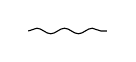
\begin{tikzpicture}
    \draw[decorate,decoration={snake,amplitude=1pt}] (0,0) -- (1,0);
\end{tikzpicture}}. Scalars have momentum. Fermions and antifermions have spin and momentum. Photons have polarisation and momentum.

We wish to find the scattering amplitude for a general process of the following form:
\begin{figure}[H]
    \centering
    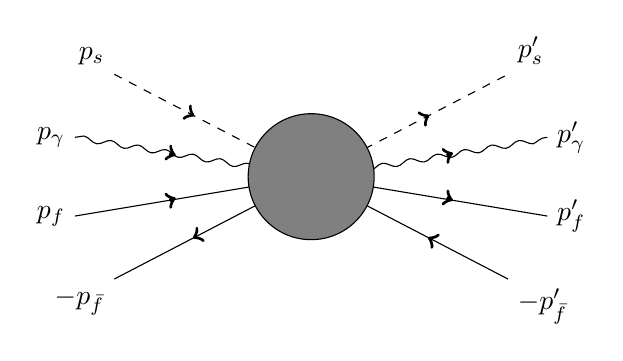
\begin{tikzpicture}
        \draw[dashed] (-2.5,1.3) node[above left] {\(p_s\)} -- (0,0) -- (2.5,1.3) node[above right] {\(p_s'\)};
        \draw[decorate,decoration={snake,amplitude=1pt}] (-3,0.5) node[left] {\(p_\gamma\)} -- (0,0) -- (3,0.5) node[right] {\(p_\gamma'\)};
        \draw (-3,-0.5) node[left] {\(p_f\)} -- (0,0) -- (3,-0.5) node[right] {\(p_f'\)};
        \draw (-2.5,-1.3) node[below left] {\(-p_{\bar{f}}\)} -- (0,0) -- (2.5,-1.3) node[below right] {\(-p_{\bar{f}}'\)};

        \draw[very thick,->] (-1.5,0.78) -- (-1.485,0.7722);
        \draw[very thick,<-] (1.5,0.78) -- (1.485,0.7722);
        \draw[very thick,->] (-1.8,0.3) -- (-1.72,0.27);
        \draw[very thick,<-] (1.8,0.3) -- (1.72,0.27);
        \draw[very thick,<-] (-1.5,-0.78) -- (-1.485,-0.7722);
        \draw[very thick,->] (1.5,-0.78) -- (1.485,-0.7722);
        \draw[very thick,->] (-1.8,-0.3) -- (-1.72,-0.27);
        \draw[very thick,<-] (1.8,-0.3) -- (1.72,-0.27);

        \fill[gray] (0,0) circle (0.8);
        \draw (0,0) circle (0.8);
    \end{tikzpicture}
\end{figure}
Note that inside the Feynman diagram there are various propagators and matrices. Since the action is commuting and fermions are anticommuting, fermions must come in pairs at vertices. Fermion lines thus make a continous line.

The Feynman rules for doing so are as follows:
\begin{enumerate}
    \item Draw all diagrams to relevant order in a coupling constant.
    \item Label the external lines and assign momenta.
    \item Label each internal line with the appropriate wavefunction:
        \begin{table}[H]
            \centering
            \begin{tabular}{lcc}
                Field       & Incoming                         & Outgoing \\
                \midrule
                Fermion     & \(u_s(p_f)\)                     & \(\overline{u}_s(p_f')\) \\
                Antifermion & \(\overline{v}_s(p_{\bar{f}})\)  & \(v_s(p_{\bar{f}}')\) \\
                Scalar      & \(1\)                            & \(1\) \\
                Photon      & \(\epsilon^*_\lambda(p_\gamma)\) & \(\epsilon_\gamma(p_\gamma')\)
            \end{tabular}
        \end{table}
    \item Add a propagator for each internal line:
        \begin{table}[H]
            \centering
            \begin{tabular}{lc}
                Field       & Propagator \\
                \midrule
                Fermion     & \(\displaystyle\frac{-i(-\slashed{k}+m)}{k^2+m^2-i\epsilon}\) \\
                Scalar      & \(\displaystyle\frac{-i}{k^2+m^2-i\epsilon}\) \\
                Photon      & \(\displaystyle\frac{-i\eta^{ab}}{k^2-i\epsilon}\)
            \end{tabular}
        \end{table}
    \item Determine the symmetry factor and divide by it.
    \item Integrate over all undetermined momenta with \(\pm\int\frac{\dd[4]{k}}{(2\pi)^4}\), where \(+\) is for scalars and photons, and \(-\) is for fermions.
    \item Add all diagrams to give the total amplitude but in a way that is antisymmetric over any outgoing fermions.
\end{enumerate}

As an example consider electron positron annihilation \(e^+e^-\to\gamma\gamma\) to order \(e^2\). We have the following diagrams:

\begin{figure}[H]
    \centering
    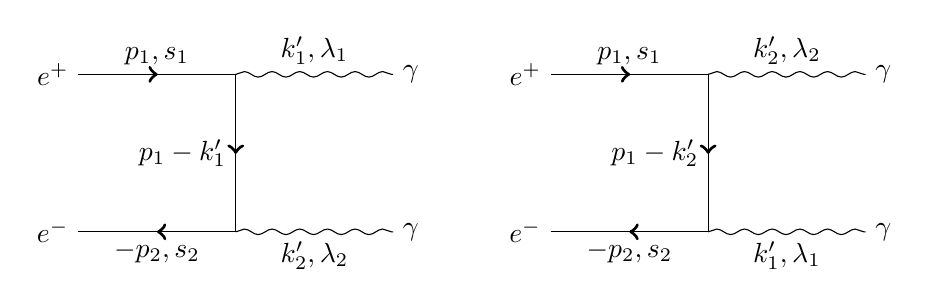
\begin{tikzpicture}
        \begin{scope}
            \draw (0,0) node[left] {\(e^-\)} -- (2,0) -- (2,2) -- (0,2) node[left] {\(e^+\)};
            \draw[decorate,decoration={snake,amplitude=1pt}] (2,0) -- (4,0) node[right] {\(\gamma\)};
            \draw[decorate,decoration={snake,amplitude=1pt}] (2,2) -- (4,2) node[right] {\(\gamma\)};
            \node[below] at (1,0) {\(-p_2,s_2\)};
            \node[above] at (1,2) {\(p_1,s_1\)};
            \node[below] at (3,0) {\(k_2',\lambda_2\)};
            \node[above] at (3,2) {\(k_1',\lambda_1\)};
            \node[left] at (2,1) {\(p_1-k_1'\)};
            \draw[very thick,<-] (1,0) -- (1.01,0);
            \draw[very thick,->] (1,2) -- (1.01,2);
            \draw[very thick,->] (2,1) -- (2,0.99);
        \end{scope}
        \begin{scope}[shift={(6,0)}]
            \draw (0,0) node[left] {\(e^-\)} -- (2,0) -- (2,2) -- (0,2) node[left] {\(e^+\)};
            \draw[decorate,decoration={snake,amplitude=1pt}] (2,0) -- (4,0) node[right] {\(\gamma\)};
            \draw[decorate,decoration={snake,amplitude=1pt}] (2,2) -- (4,2) node[right] {\(\gamma\)};
            \node[below] at (1,0) {\(-p_2,s_2\)};
            \node[above] at (1,2) {\(p_1,s_1\)};
            \node[below] at (3,0) {\(k_1',\lambda_1\)};
            \node[above] at (3,2) {\(k_2',\lambda_2\)};
            \node[left] at (2,1) {\(p_1-k_2'\)};
            \draw[very thick,<-] (1,0) -- (1.01,0);
            \draw[very thick,->] (1,2) -- (1.01,2);
            \draw[very thick,->] (2,1) -- (2,0.99);
        \end{scope}
    \end{tikzpicture}
\end{figure}
\emph{Mandelstam variables} are often used to find how these diagrams deal with momenta. The Mandelstam variables are
\begin{align}
    s &= -(p_1+p_2)^2 \quad \text{(measure of left to right momentum)}, \\
    t &= -(p_1-k_1')^2 \quad \text{(measure of momentum transfer in first diagram)}, \\
    u &= -(p_1-k_2')^2 \quad \text{(measure of momentum transfer in second diagram)}.
\end{align}
Note that since \(s+t+u=2m^2\), where \(m^2\) is the sum of the masses squared for all external particles, two of these variables fully determine the third.

Using the above Feynman rules we can then determine the transfer matrix (i.e.\ the amplitude modulo momentum conservation):
\begin{equation}
    T = e^2\epsilon_{\lambda_1}^a(k_1')\epsilon_{\lambda_2}^b(k_2')\overline{v}_{s_2}(p_2)\left[\gamma_b\frac{-(\slashed{p}_1-\slashed{k}_1')+m}{(p_1-k_1')^2+m^2-i\epsilon}\gamma_a + \gamma_a\frac{-(\slashed{p}_1-\slashed{k}_2')+m}{(p_1-k_2')^2+m^2-i\epsilon}\gamma_b\right]u_{s_1}(p_1)
\end{equation}

**Non-examinable**
In terms of Mandelstam variables, we have
\begin{equation}
    \frac{1}{4} \sum_{\text{spins}} \sum_{\lambda_1,\lambda_2}|T|^2 = e^4\Big[\underbrace{\frac{\Phi_{tt}}{(m^2-t)^2}}_{\text{first diagram}} + \underbrace{\frac{\Phi_{tu}+\phi_{ut}}{(m^2-u)(m^2-t)}}_{\text{interference cross term}} + \underbrace{\frac{\Phi_{uu}}{(m^2-u)^2}}_{\mathclap{\text{second diagram}}}\Big],
\end{equation}
where
\begin{align}
    \Phi_{tt} &= 2(tu-m^2(3t+u)-m^4), \\
    \Phi_{uu} &= 2(tu-m^2(3u+t)-m^4), \\
    \Phi_{ut} = \Phi_{tu} &= 2m^2(s-4m^2).
\end{align}
It is then an exercise in arithmetic to calculate the scattering cross section with
\begin{equation}
    \dv{\sigma}{\Omega} = \frac{1}{64\pi^2 s}|T|^2.
\end{equation}

\end{document}
